\chapter{Statistical analysis and results}
\label{chap:statandresults}

The signal and background models described in \Chapter~\ref{} are used to interpret the 35.8\fb of data which are considered in this analysis, and make meaningful statements about the existence of the Higgs boson (in its decay to two photons), and measurements of its properties.

The first step is to determine the best signal-and-background fit in the region of interest, where the floating parameters of the signal and background models are varied simultaneously in each analysis category to obtain the closest overall agreement with the data. This is described in \Sec~\ref{}, and will establish the existence of a strong signal. Next, the significance of this signal is established and quantified, and used to reject the hypothesis that there exists no Higgs boson. This procedure and the result are described in \Sec~\ref{}. Finally, having established the existence of the Higgs boson decaying to photons, the final step is to make measurements of its properties. These measurements are described in \Sec\s~\ref{} and~\ref{}.



\section{Best fit of models to the data}

The \mgg distributions obtained from the data in each analysis category are fitted with a model consisting of signal and background components. 

For the signal component, we use the parametric model described in \Sec~\ref{}. The values of the individual parameters of \DCBpG functions used to produce the models for each process and each category are fixed: specifically, this refers to the eight \DCBpG parameters for each of the \RV and \WV scenarios, as well as their mixing fractions. The parameters which are allowed to vary are the nuisance parameters introduced into the signal modelling to account for systematic uncertainties (\Sec~\ref{}) as well as the \mH parameter, which in this case is treated like the other nuisance parameters, or \emph{profiled}. The \POI is the signal strength $\mu = \sigma^{H} / \sigma^{H}_{SM}$, , where in this context $\sigma^H$ is the observed Higgs boson cross section, and  $\sigma^H_{SM}$ is the \SM \crosssection. The scales all the signal models for each process uniformly in the fit. This means that the contribution to the overall signal model from each process remains in proportion to what is predicted by the \SM, but the overall normalisation of all signal models can be varied. 
For the background component, the choice of background function in each analysis category is treated as a discrete nuisance parameter when fitting, as described in \Sec~\ref{}. In addition, the individual parameters of the candidate functions are also floating nuisance parameters. 

The fit is obtained by minimising the twice the negative log-likelihood: $ -2 \ln \mathcal{L}(\mu,\mathbf{n}| \mathbf{x}$. The likelihood function $\mathcal{L}(\mu,\mathbf{n})$ represents the probability of obtaining the values of \POI $\mu$ and nuisance parameters $\mathbf{n}$ given observed data $\mathbf{x}$. The overall negative log-likelihoods is obtained by taking the sum of the likelihood for each individual analysis category.
The best-fit values of the \POI and nuisance parameters are denoted as $\hat{mu}$ and $\hat{\mathbf{n}}$, and correspond to :
\begin{equation}
(\hat{mu}, \hat{\mathbf{n}}) = { (mu,\mathbf{n}) : -2 \ln \mathcal{L}(\hat{\mu},\hat{\mathbf{n}}| \mathbf{x} = \inf _{\mu,\mathbf{n}}(-2 \ln \mathcal{L}(\mu,\mathbf{n}| \mathbf{x}) },
\end{equation}
where $\inf_{ \mu,\mathbf{n}}$ represents the \emph{infimum} over all allowed values of $\mu$ and $\mathbf{n}$. This technique can be generalised for an arbitrary number of \POI\s. 

In general, the \NLL cannot be minimized analytically. Therefore, it is minimised numerically using the \Minuit package~\cite{}. The resulting parametrisations are shown with the data for each analysis category separately in \Fig\s~\ref{fig:statandresults:s_b_fits} and~\ref{fig:statandresults:s_b_fits_bis}. The combined parametrisations and data  resulting from a direct sum of each category is shown in \Fig~\ref{fig:statandresults:s_b_fits_direct_sum}, while the sum weighted by the $S/(S+B)$ in $\pm \effSigma$ around the best-fit $\mH$ is shown in \Fig~\ref{fig:statandresults:s_b_fits_s_sb_sum}. The best-fit value of the \POI \mu is $\hat{\mu}= 0.95$, indicating a string \SM-like Higgs boson signal. 


\begin{figure}[ht!]
\centering
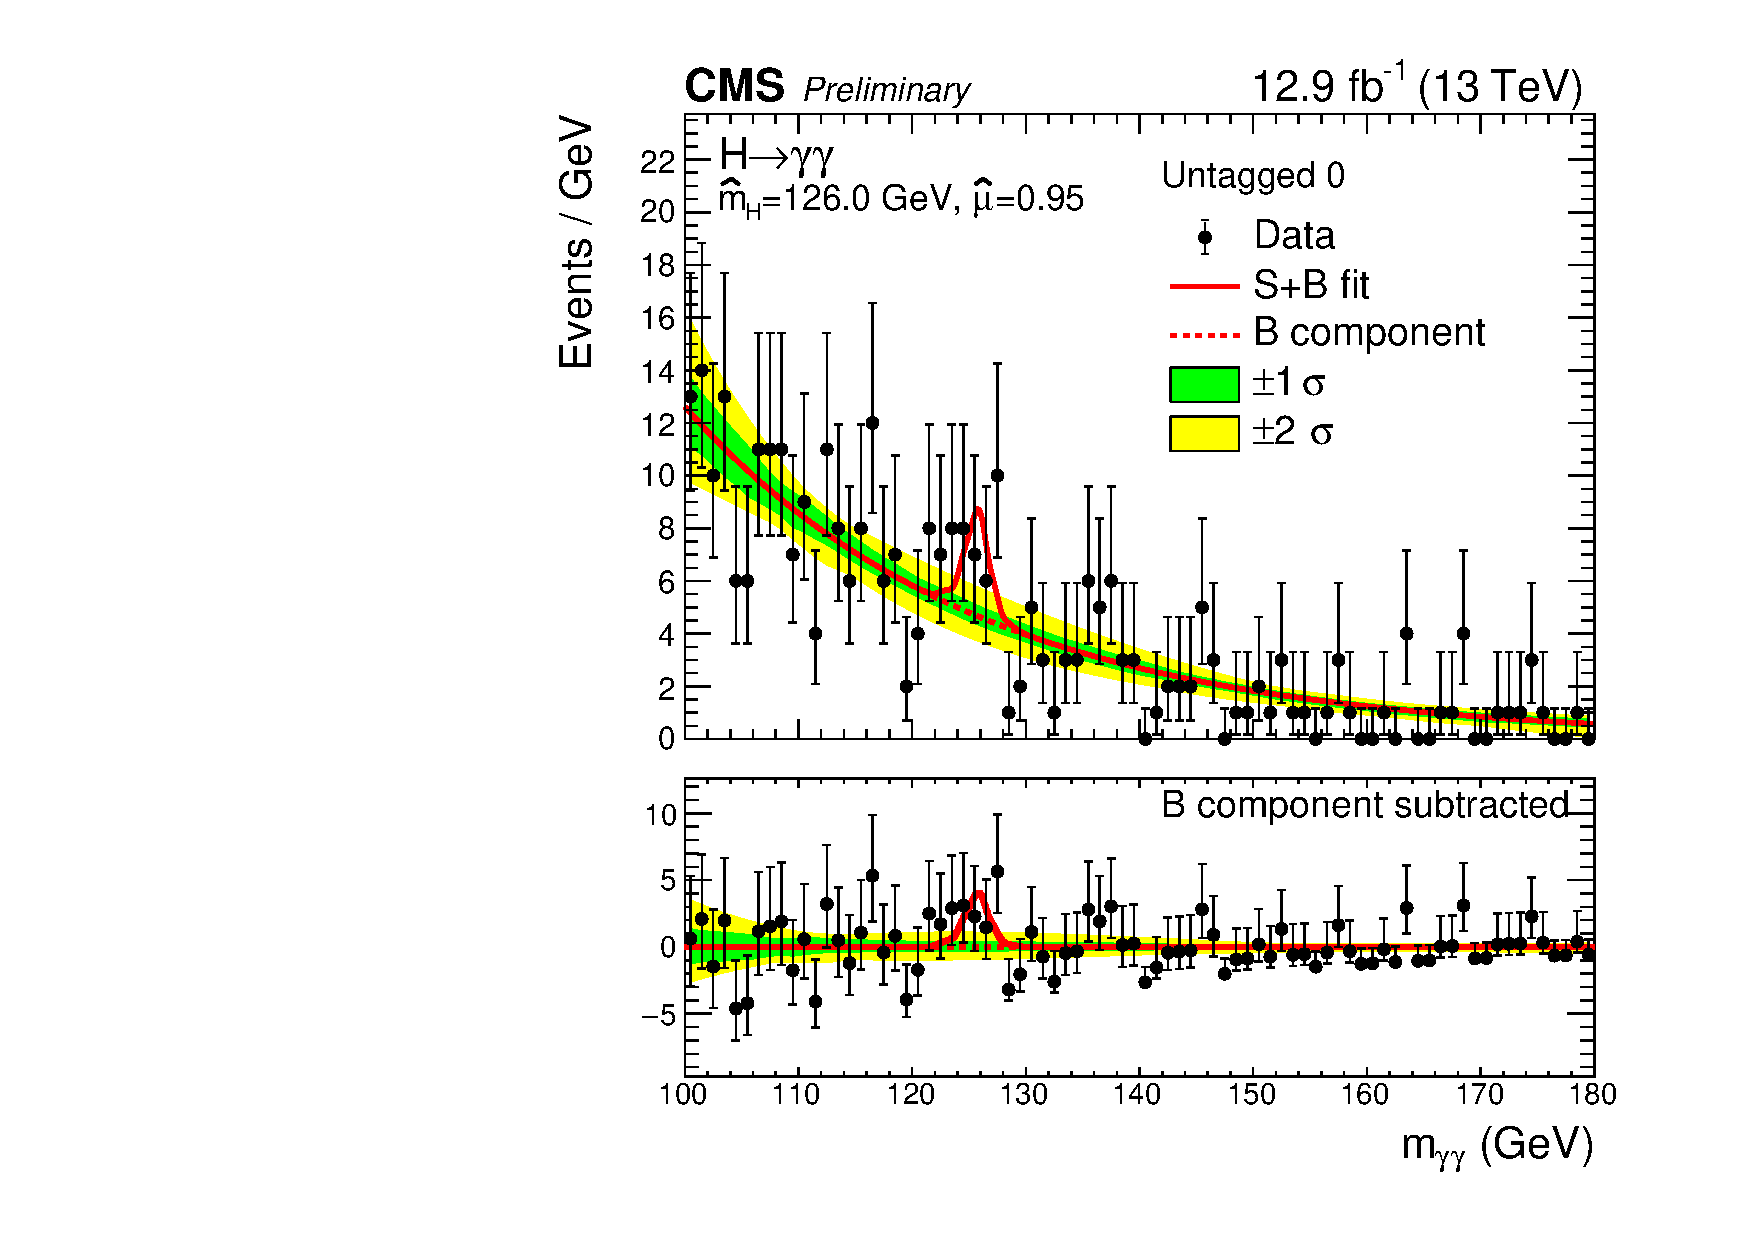
\includegraphics[width=0.45\textwidth]{statandresultsFigures/S_SB_ProfileMH_UntaggedTag_0_13TeV.pdf} 
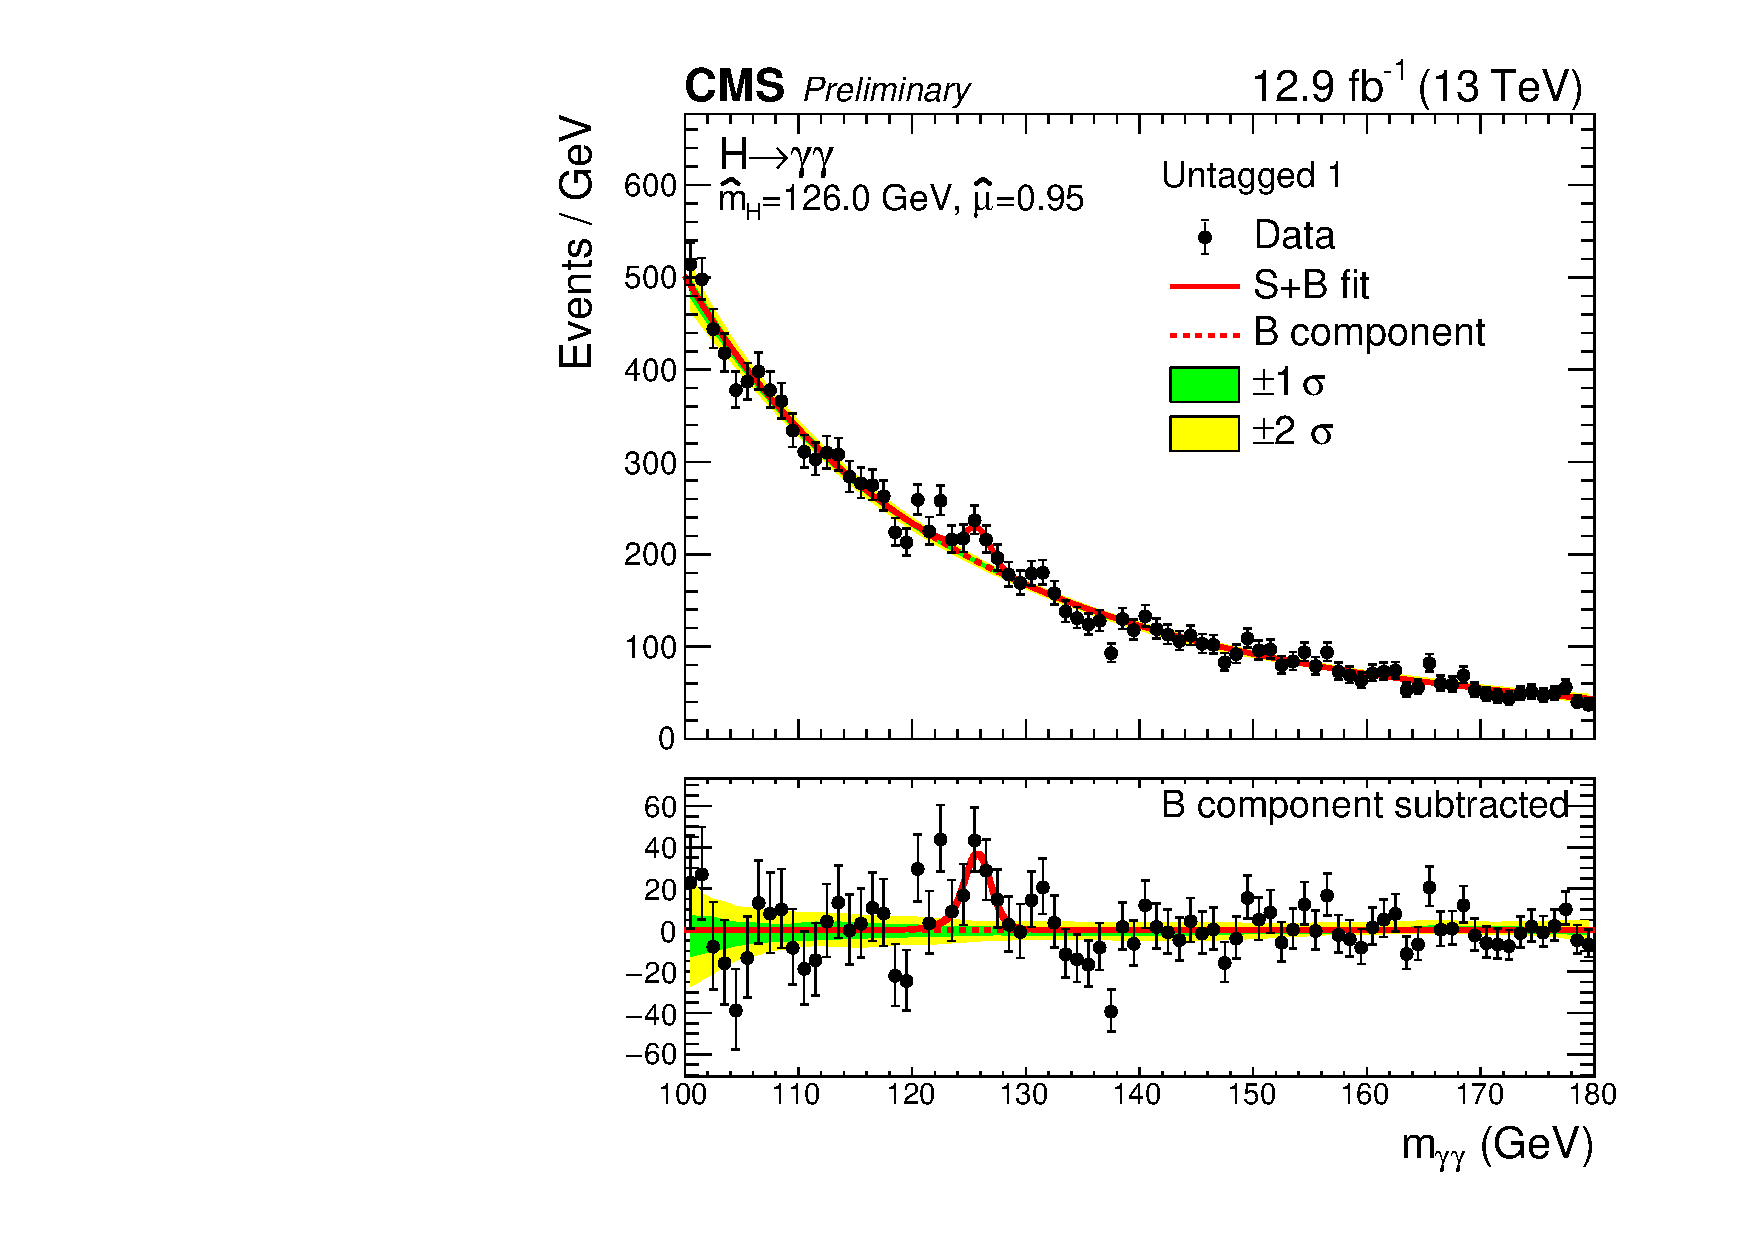
\includegraphics[width=0.45\textwidth]{statandresultsFigures/S_SB_ProfileMH_UntaggedTag_1_13TeV.pdf}\\ 
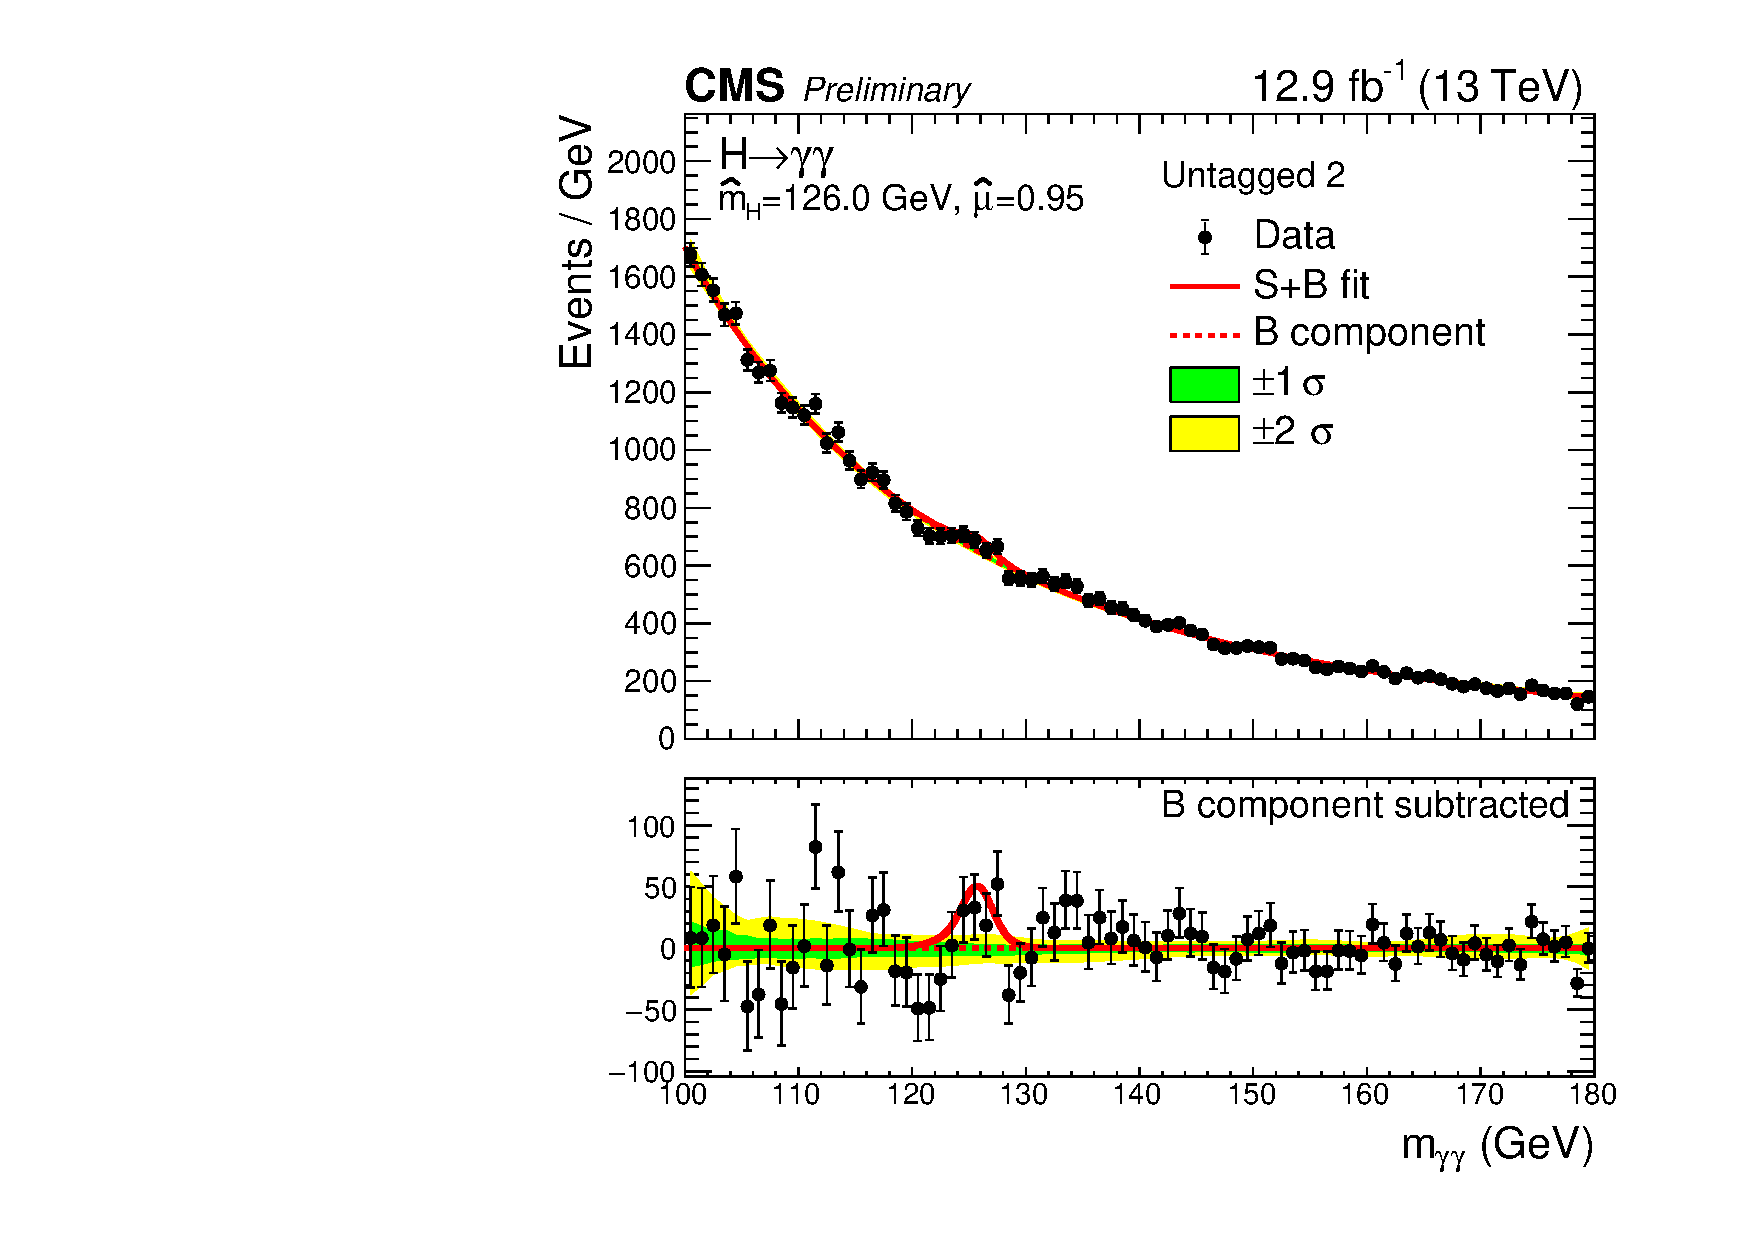
\includegraphics[width=0.45\textwidth]{statandresultsFigures/S_SB_ProfileMH_UntaggedTag_2_13TeV.pdf} 
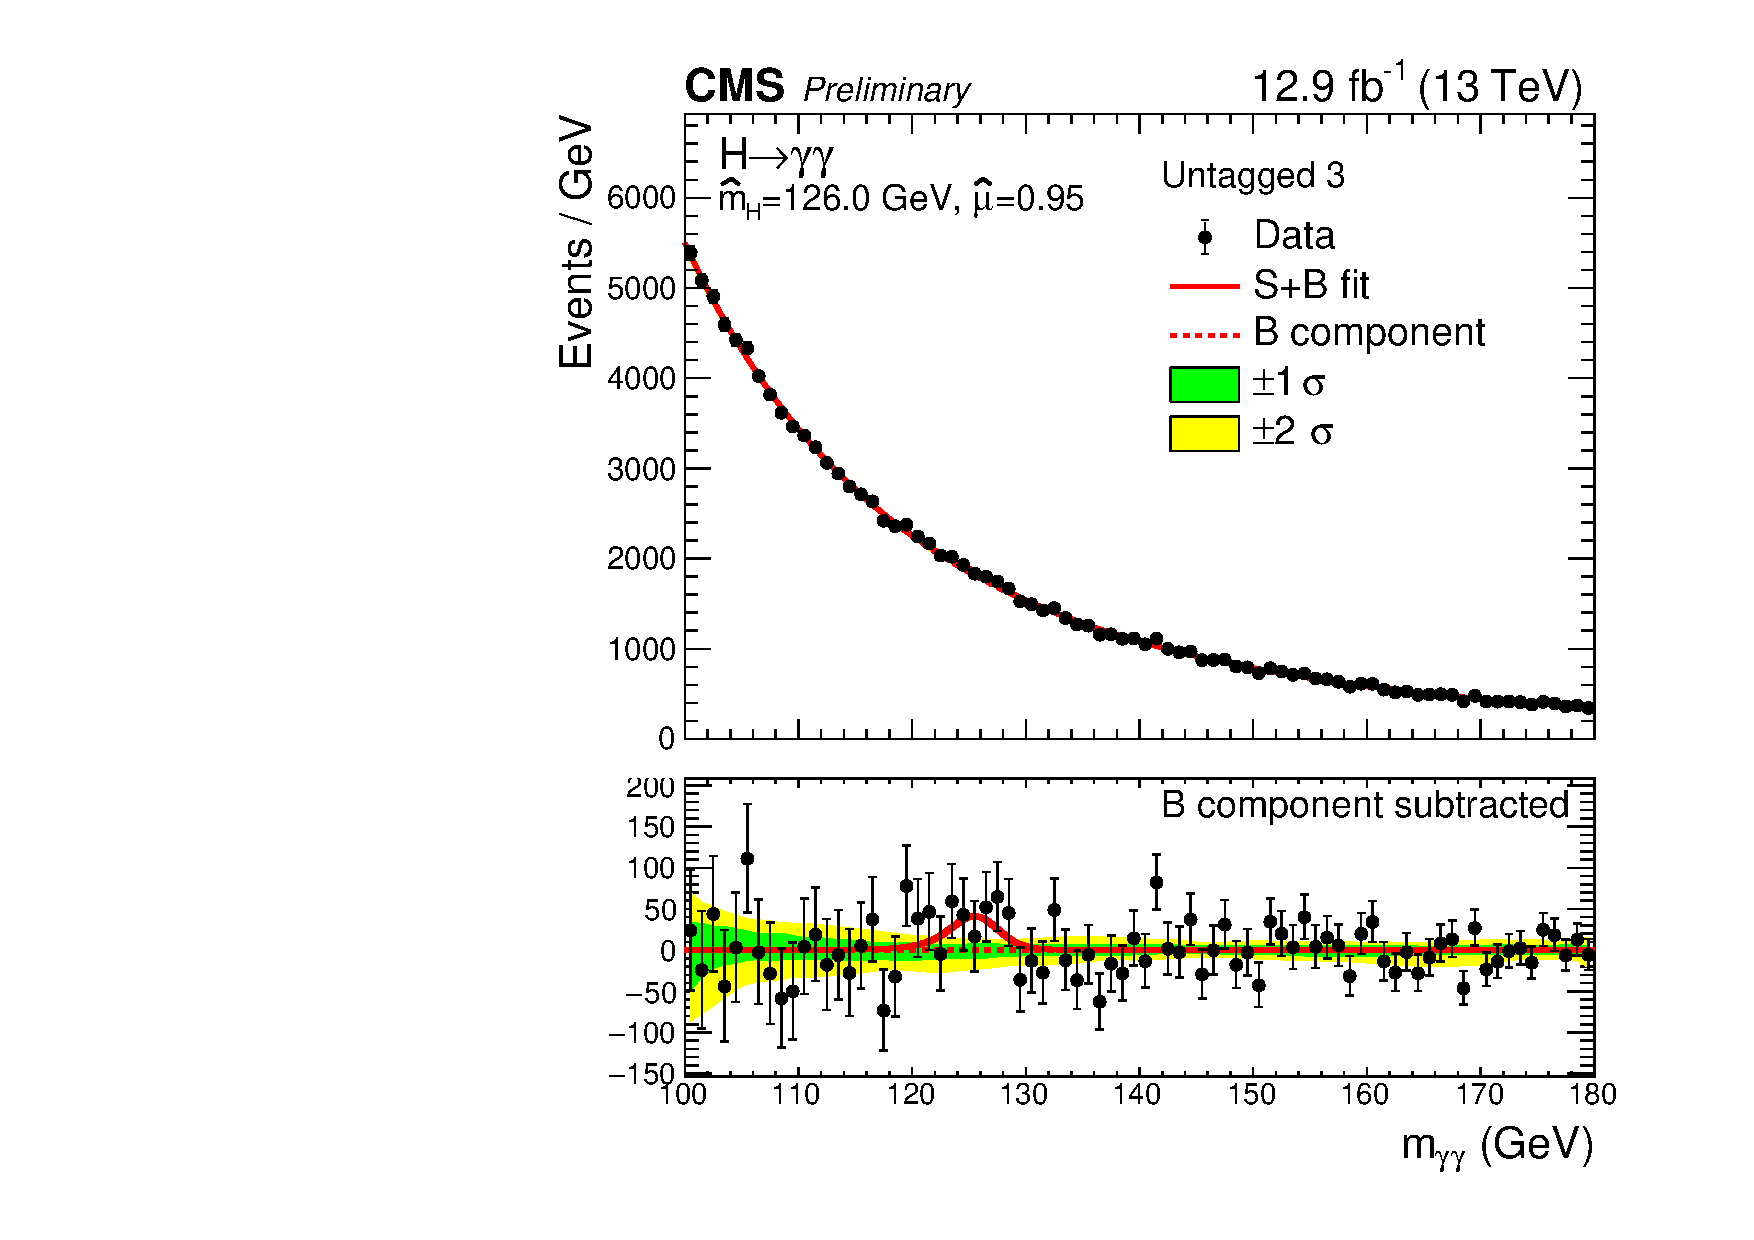
\includegraphics[width=0.45\textwidth]{statandresultsFigures/S_SB_ProfileMH_UntaggedTag_3_13TeV.pdf} \\
\caption{The \mgg distribution for the \Untagged analysis categories. The data points in shown black, while the signal-plus-background fit of all analysis categories simultaneously is shown as a solid red line. The background-only fit is shown as a dashed red line, with the green and yellow bands denoting the $1\sigma$ and $2\sigma$ uncertainties on the background shape respectively.}

\label{fig:statandresults:s_b_fits}
\end{figure}

\begin{figure}[ht!]
\centering
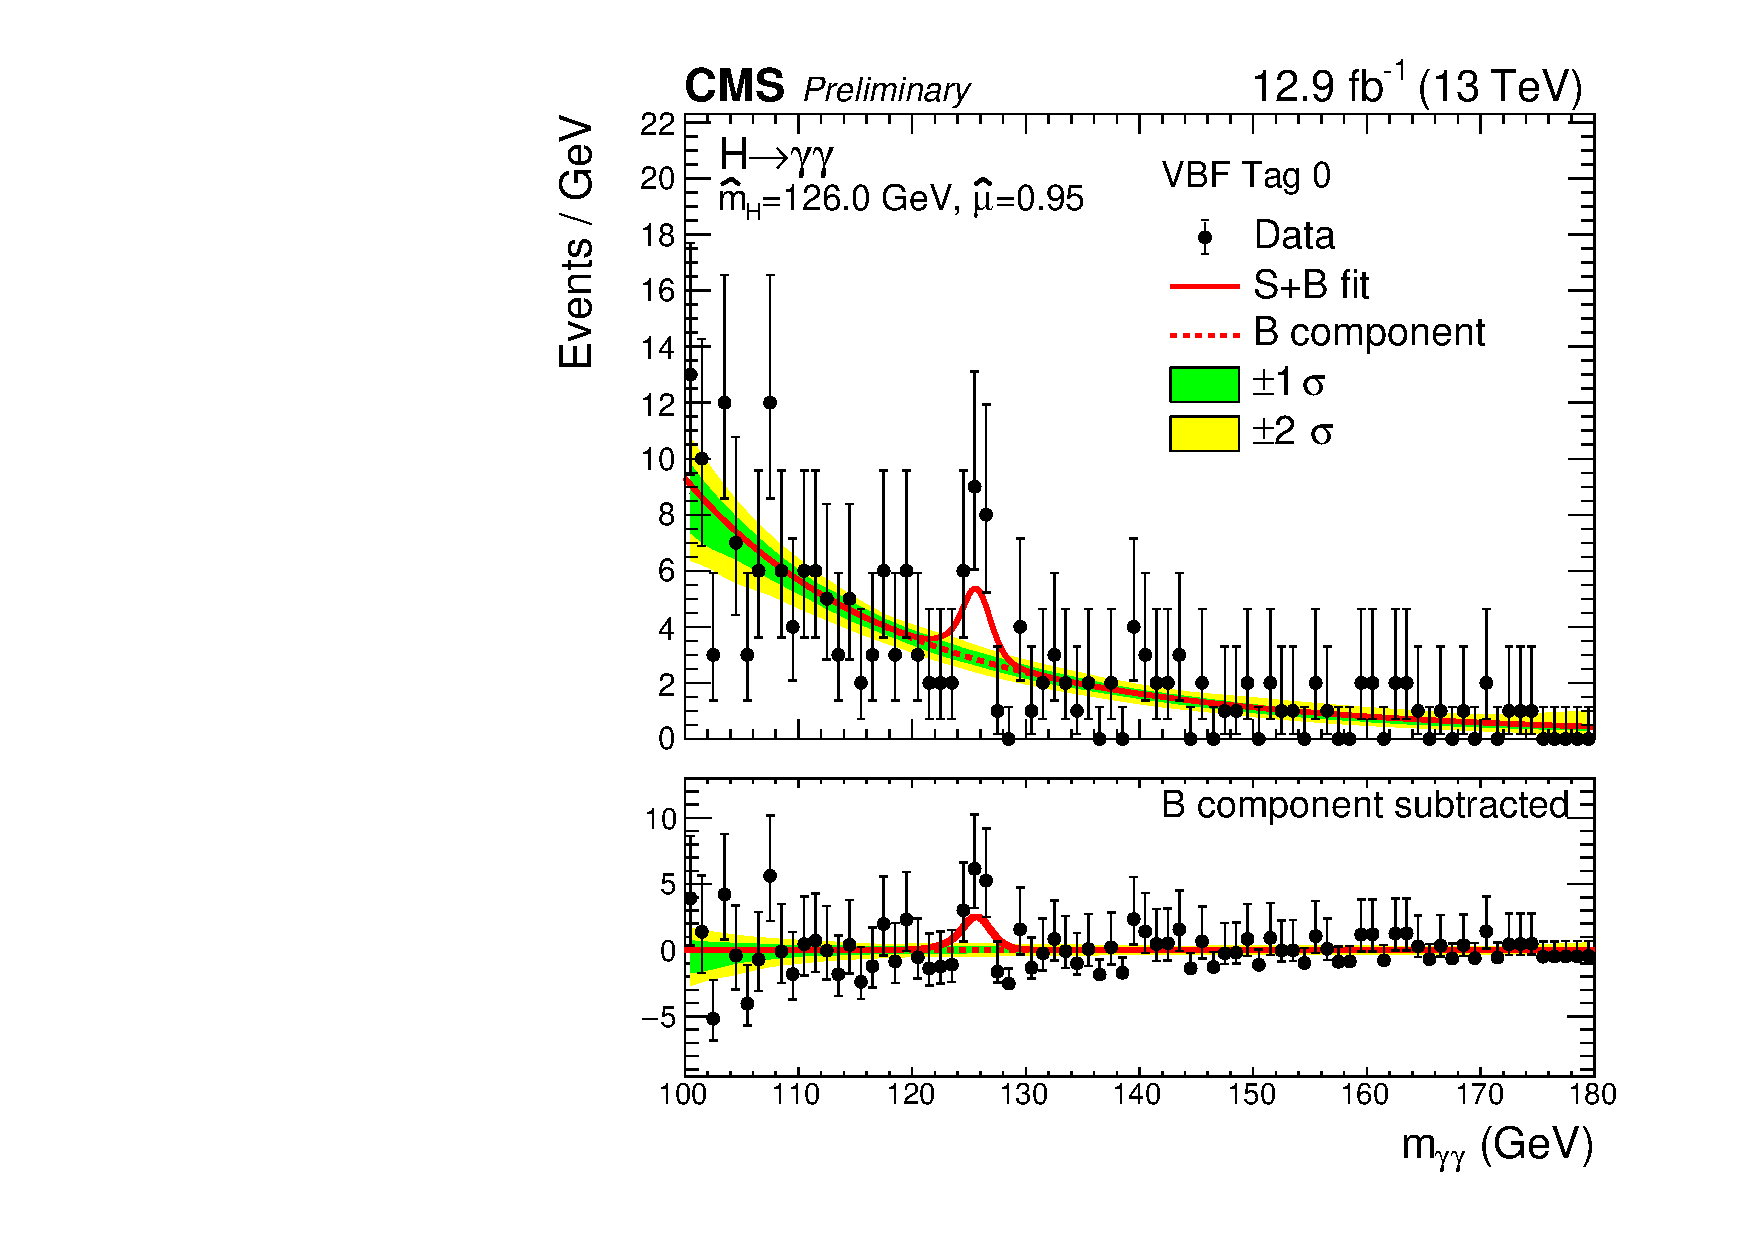
\includegraphics[width=0.45\textwidth]{statandresultsFigures/S_SB_ProfileMH_VBFTag_0_13TeV.pdf} 
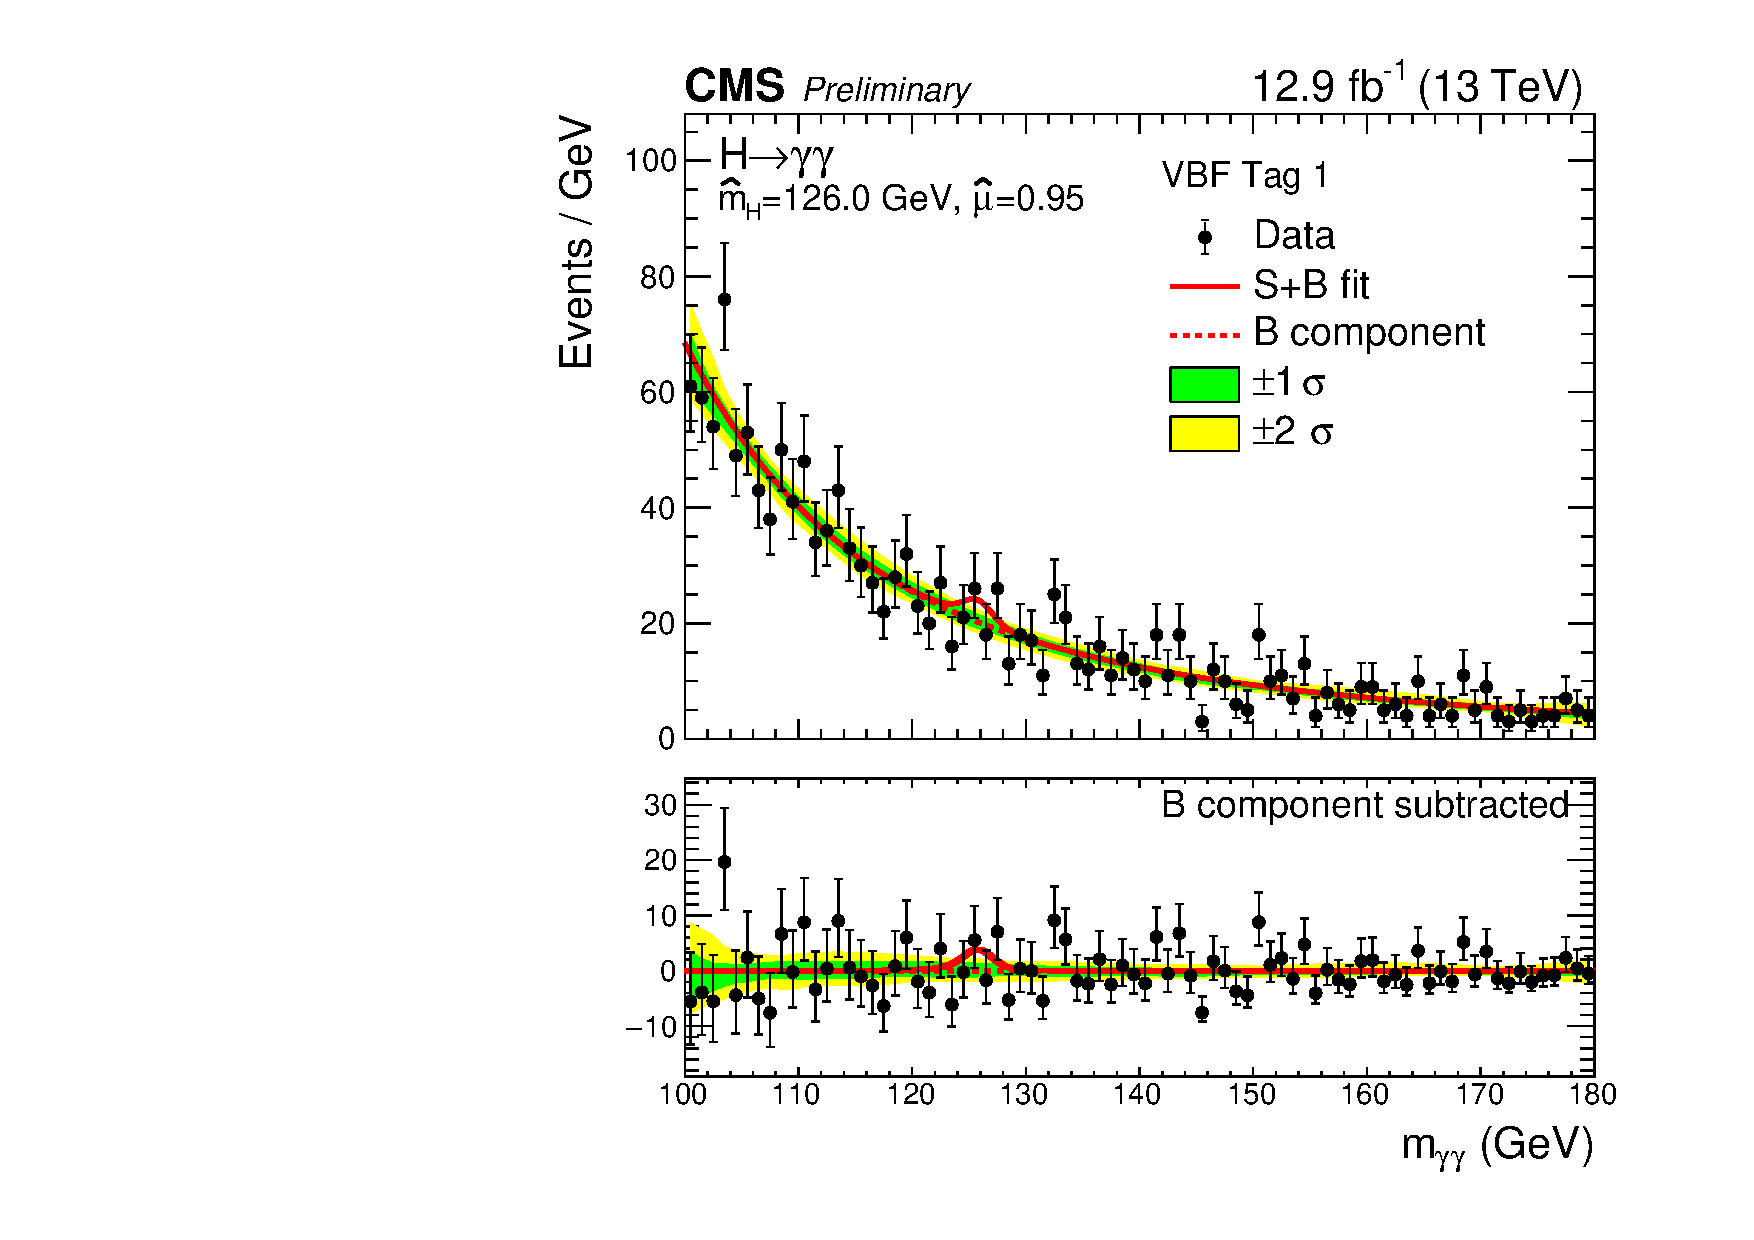
\includegraphics[width=0.45\textwidth]{statandresultsFigures/S_SB_ProfileMH_VBFTag_1_13TeV.pdf} 
%\includegraphics[width=0.3\textwidth]{statandresultsFigures/S_SB_ProfileMH_VBFTag_2_13TeV.pdf} 
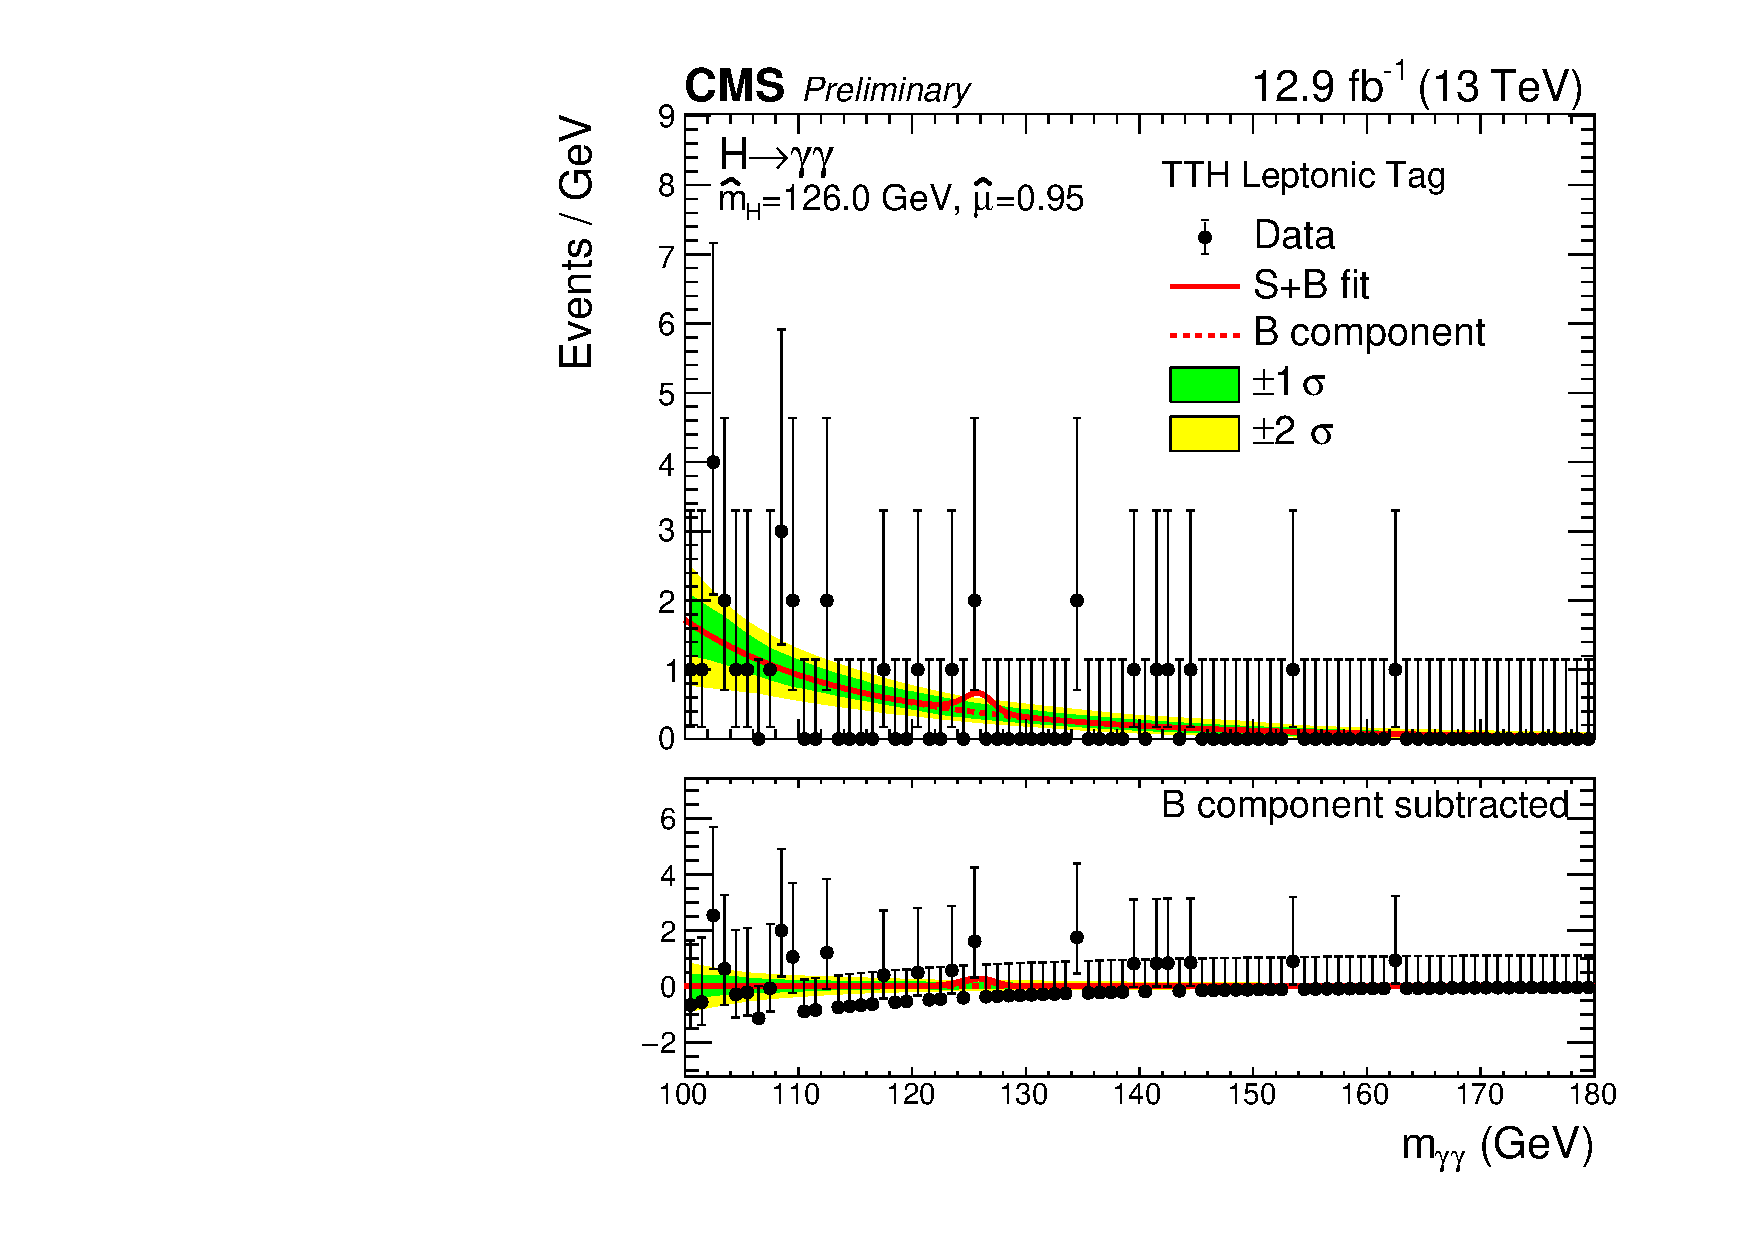
\includegraphics[width=0.45\textwidth]{statandresultsFigures/S_SB_ProfileMH_TTHLeptonicTag_13TeV.pdf} 
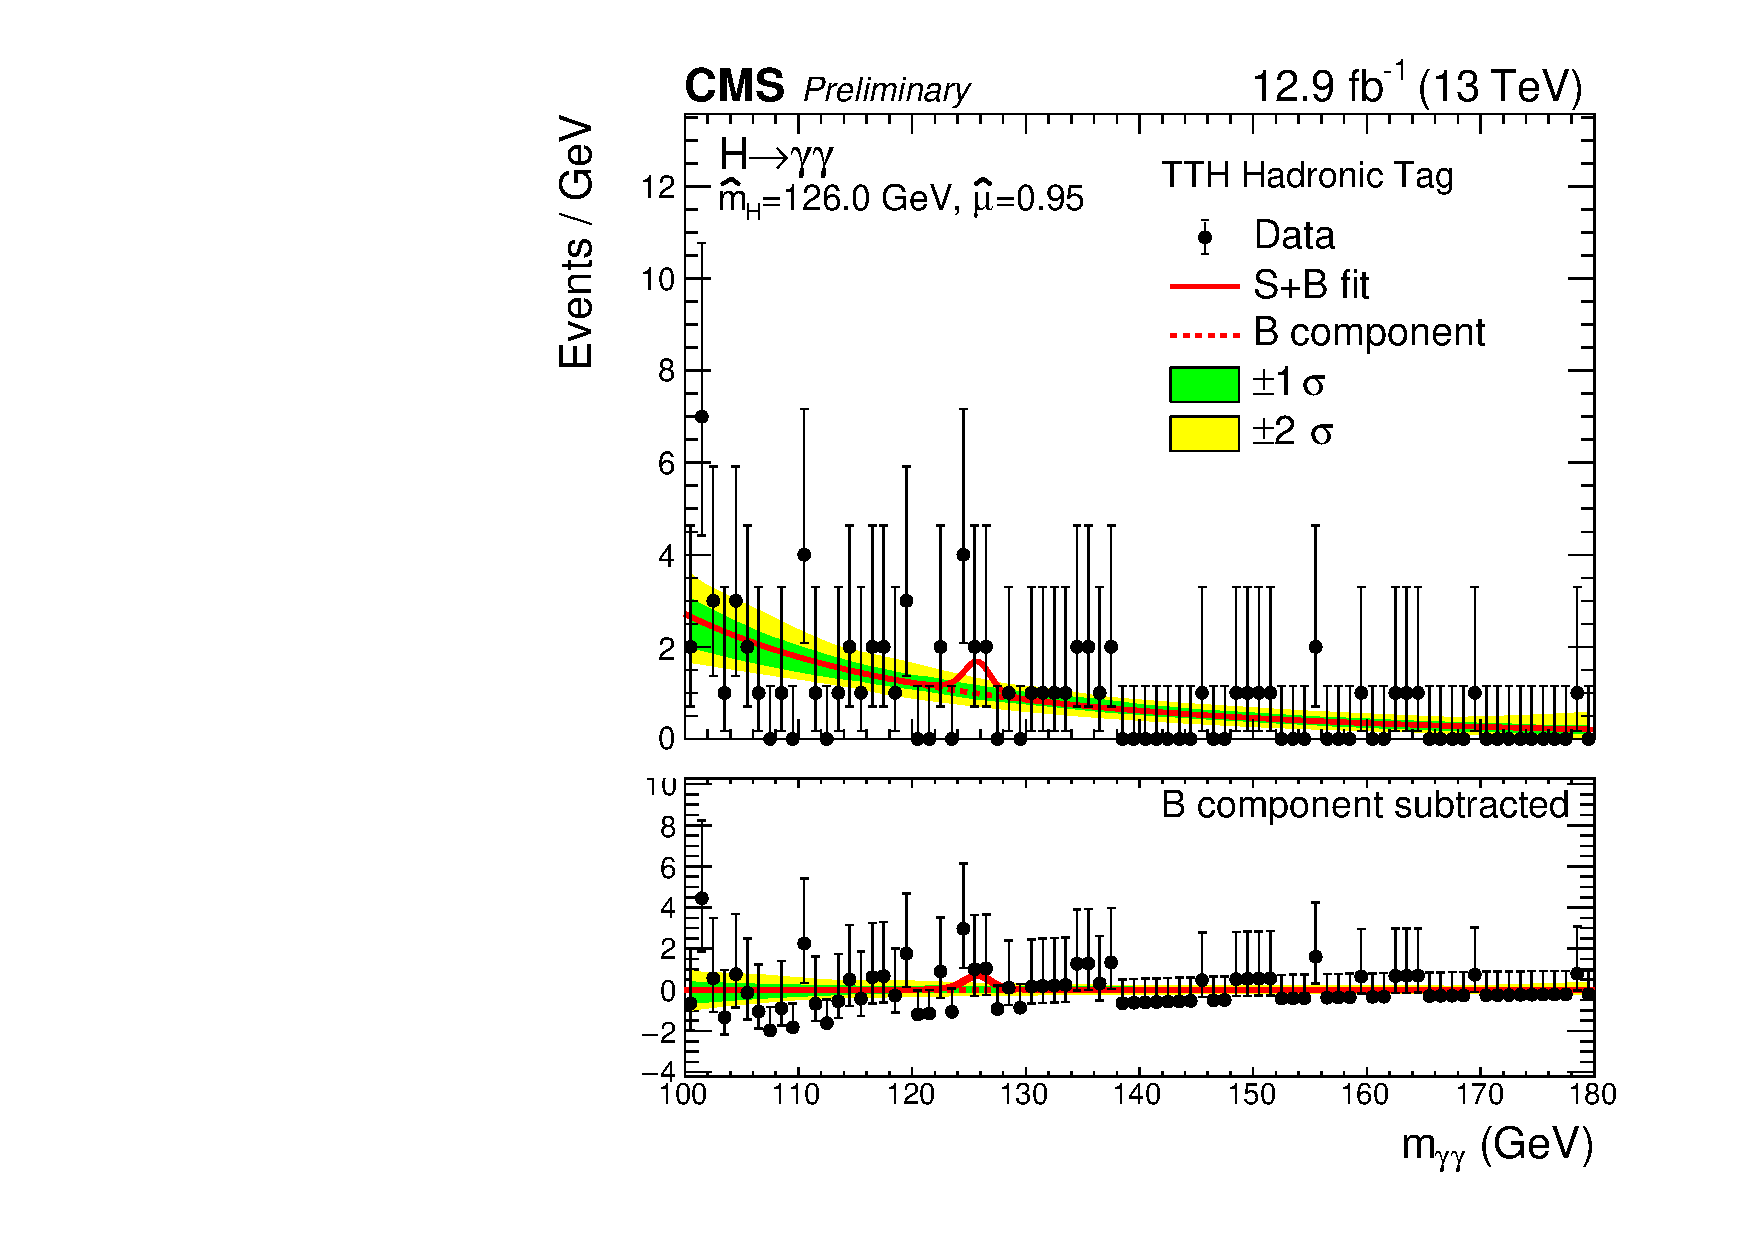
\includegraphics[width=0.45\textwidth]{statandresultsFigures/S_SB_ProfileMH_TTHHadronicTag_13TeV.pdf} \\
%\includegraphics[width=0.3\textwidth]{statandresultsFigures/S_SB_ProfileMH_VHLeptoniclooseTag_13TeV.pdf} 
%\includegraphics[width=0.3\textwidth]{statandresultsFigures/S_SB_ProfileMH_VHMetTag_13TeV.pdf} 
%\includegraphics[width=0.3\textwidth]{statandresultsFigures/S_SB_ProfileMH_VHHadronicTag_13TeV.pdf} \\
%\includegraphics[width=0.3\textwidth]{statandresultsFigures/S_SB_ProfileMH_WHLeptonicTag_13TeV.pdf} 
%\includegraphics[width=0.3\textwidth]{statandresultsFigures/S_SB_ProfileMH_ZHLeptonicTag_13TeV.pdf} 
\caption{The \mgg distribution for the and \VBFTag a\TTHTag analysis categories. The data points in shown black, while the signal-plus-background fit of all analysis categories simultaneously is shown as a solid red line. The background-only fit is shown as a dashed red line, with the green and yellow bands denoting the $1\sigma$ and $2\sigma$ uncertainties on the background shape respectively.}

\label{fig:statandresults:s_b_fits_bis}
\end{figure}

\begin{figure}[ht!]
\centering
\subfloat[Direct sum]{
 \label{fig:statandresults:s_b_fits_direct_sum}
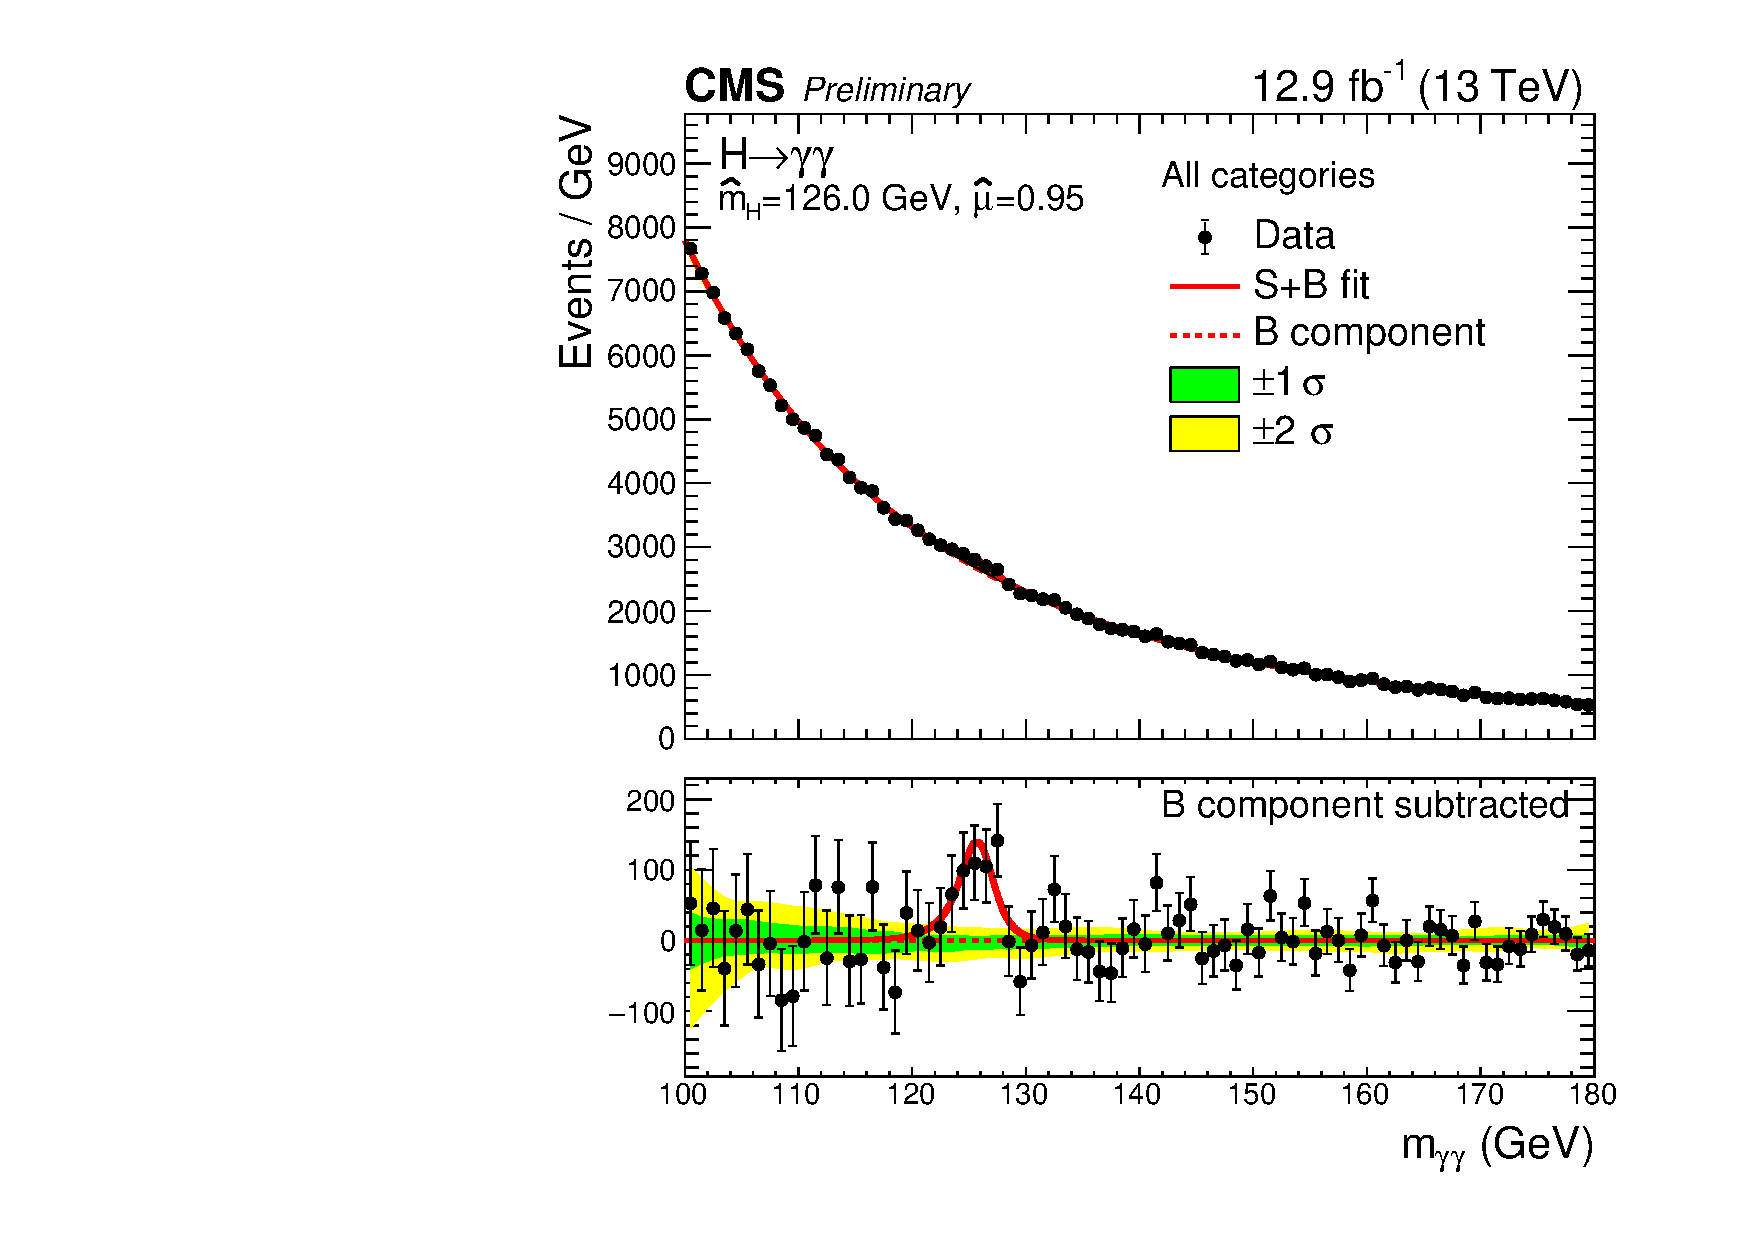
\includegraphics[width=0.55\textwidth]{statandresultsFigures/S_SB_ProfileMH_combcat_unweighted.pdf}}\\
\subfloat[S/(S+B) weighted sum]{
 \label{fig:statandresults:s_b_fits_s_sb_sum}
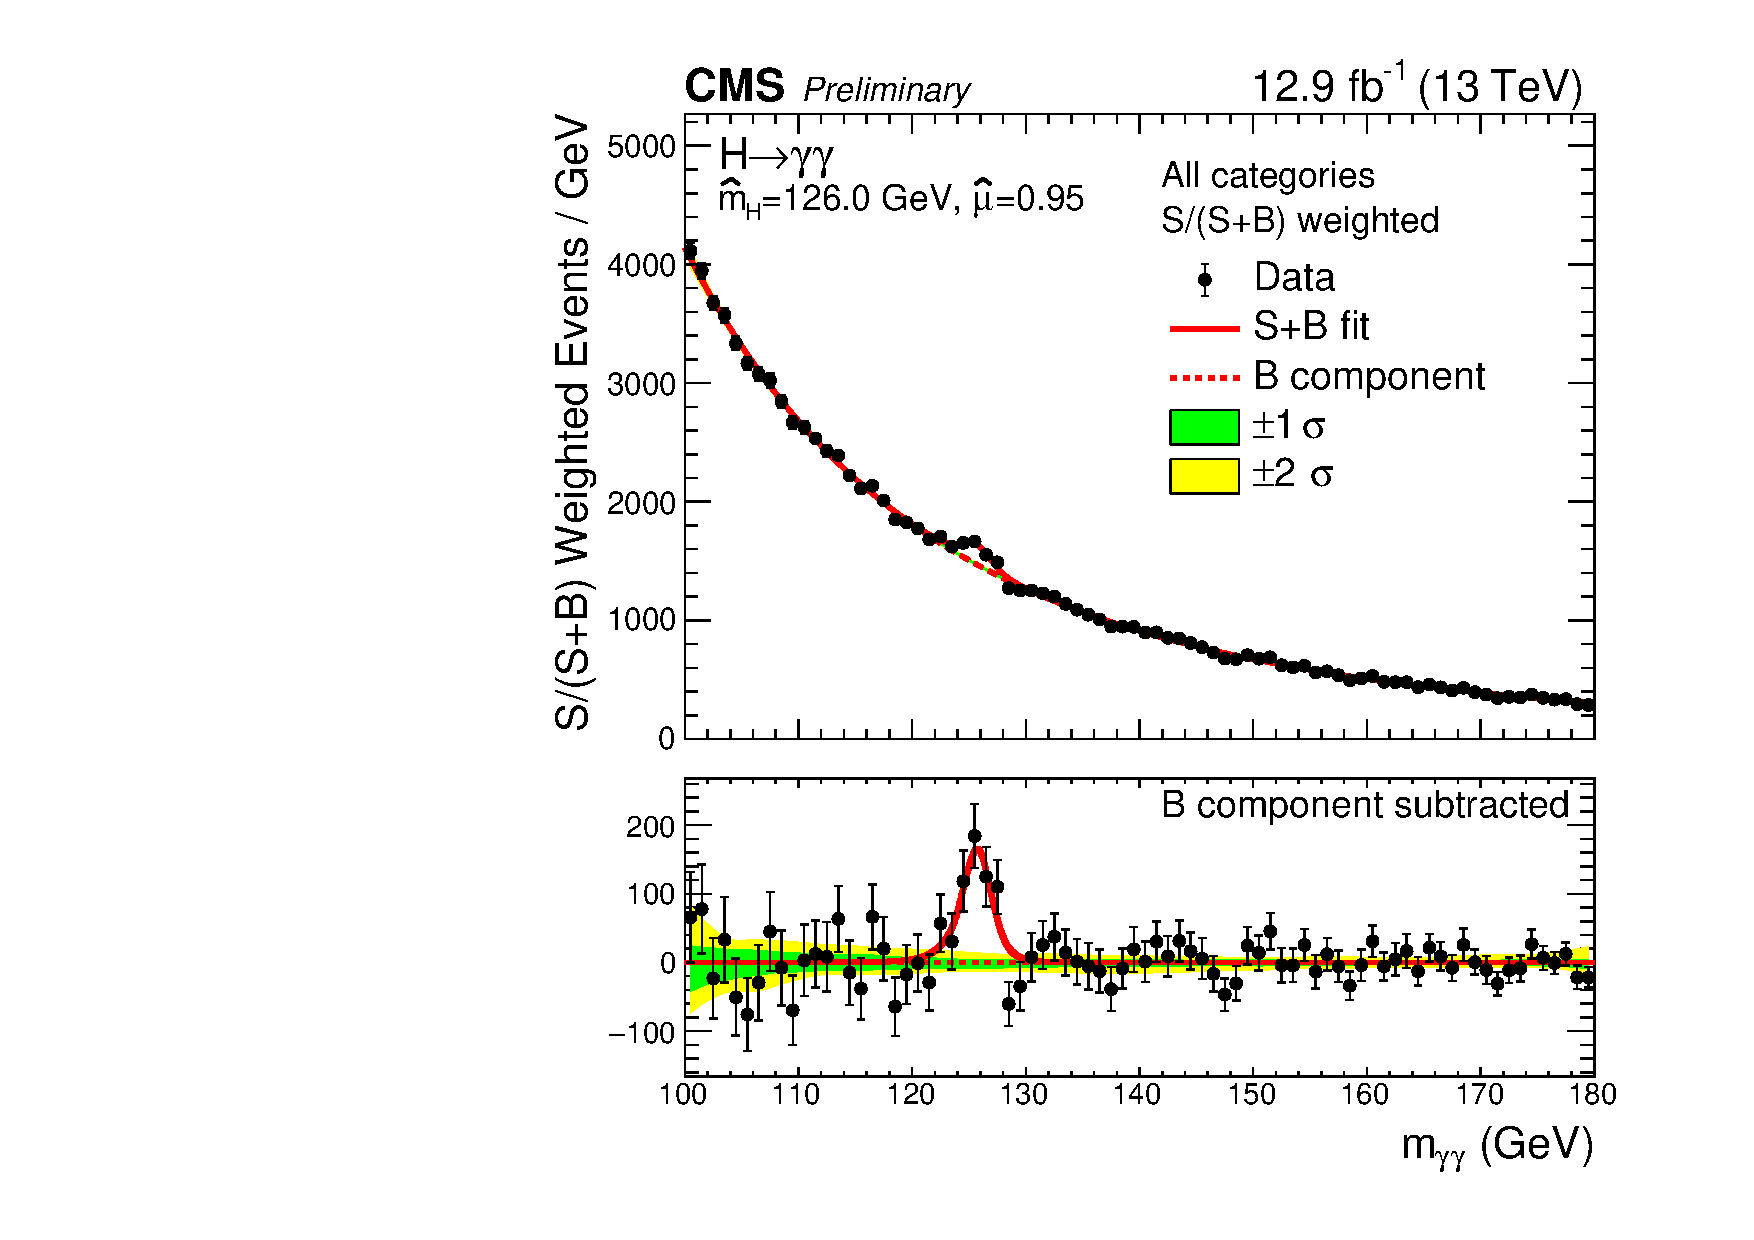
\includegraphics[width=0.55\textwidth]{statandresultsFigures/S_SB_ProfileMH_combcat_weighted.pdf}}
\caption{The \mgg distribution for all categories combine, either using a direct sum (a) or a sum weighted by the $S/(S+B)$ in $\pm \effSigma$ around the best-fit value of \mH (b) . The data points in shown black, while the signal-plus-background fit of all analysis categories simultaneously is shown as a solid red line. The background-only fit is shown as a dashed red line, with the green and yellow bands denoting the $1\sigma$ and $2\sigma$ uncertainties on the background shape respectively.}

\label{fig:statandresults:s_b_fits_sum}
\end{figure}


\section{Significance of observation}


Given the best-fit value of the \POI \mu is $\hat{\mu}= 0.95$ in \Sec~\ref{}, it is necessary to determine the degree of certainty with which the hypothesis that there is no Higgs boson can be rejected , in favour of an alternative hypothesis which is that a \SM-like Higgs boson exists. A frequentist approach is used. The hypotheses can be formulated in terms of the signal strength: the null hypothesis $H_{0}$ corresponds to the case where $\mu=0$, while the alternative hypothesis $H_{\mu}$ corresponds to $\mu > 0$. 

A statistical test is constructed by specifying a critical region $w$ of the data space, such that for a given set of observed data $\mathbf{x}$:
\begin{equation}
P(\mathbf{x} \in w | H_{0} ) \leq \alpha,
\end{equation}

where  $P(\mathbf{x} \in w | H_{0} ) $ is the probability (assuming that $H_{0}$ is correct), of observing the data inside the critical region $w$, and $\alpha$ is a small predetermined threshold. The statistical power $\beta$ of the test is the probability of to accept $H_{0}$ when it was false and the alternative $H_{\mu} $ was true. This is given by

\begin{equation}
P(\mathbf{x} \in  w | H_{\mu} ) = 1 - \beta,
\end{equation}.

The critical region should be chosen such that the power $\beta$ of the test is maximised for a given $\alpha$, to ensure that if $\mathbf{x} \in w$, then $H_{0}$ has a low probability of being true while $H_{\mu}$ has a high probability of being true.  

A common choice, which is found to maximise $\beta$~\cite{}, is to define the critical region in terms of a test statistic $q_{\mu}$, the \DNLL,  which is related to the \NLL defined in \Sec~\ref{} :
\begin{equation}
q_{\mu} = \begin{cases} 
  -2 \ln \mathcal{L}(\mu,\hat{\mathbf{n}}_{\mu}| \mathbf{x}- \ln\mathcal{L}(\hat{\mu},\hat{\mathbf{n}}| \mathbf{x} ) & \text{when } \hat{\mu} \geq 0, \\
  0 & \text{when } \hat{\mu} < 0, 
  \end{cases}
\end{equation}

where the symbol $\hat{\mathbf{n}}_{\mu}$ denotes the best-fit values $\mathbf{n}$ for a fixed value of $\mu$. When trying to exclude hypothesis $H_{0}$, the test statistic $q_0$ in particular should be used to define a critical region. In the limit of a large sample of data, the probability distribution function of the test statistic $f(q_0)$ is Gaussian. The fact that $q_{0} =0$ for $\hat{\mu} < 0$ reflects the fact that only excesses in the data are regarded as significant. This simplifies the definition of the critical region, since increasingly large values of $q_0$ indicate increasing incompatibility with $H_{0}$, and therefore we only need to consider right-hand tail of $f(q_0)$ when assessing probabilities. Assuming $H_{0}$, the probability of of obtaining a value of $q^{\mathbf{x}}_{0}$ (corresponding to observed data $ \mathbf{x}$) or higher is given by the integral of $f(q_0)$ from $q^{\mathbf{x}}_{0}$ to infinity. This probability is commonly referred to as the \pvalue. We can therefore define the critical region as:  
such that:

\begin{equation}
w = \{ \mathbf{x} : \int_{q^{\mathbf{x}}_{0}}^{+\infty} f(q_{0}) dq_0  \leq \alpha \},
\end{equation}

In particle physics experiments, the threshold $\alpha$ to reject the null hypothesis is $2.87 \times 10^{-7}$. If expressed as the number of standard deviations that a Gaussian-distributed variable would fluctuate to give the same \pvalue, then this threshold is $5\sigma$.

The \pvalue of the observed data can be evaluated separately for different assumption about the value of \mH. In this case, the value of \mH is fixed to the given value rather than profiled in the \DNLL minimisation. The result of a scan of the \pvalue\s as a function of \mH in 0.1\GeV steps is shown in~\ref{fig:statandresults:pval}. The black solid line represents the \pvalue scan for the observed data. The dashed lines represent the expected \pvalue\s for a \SM Higgs boson. These are obtained by generating an Asimov dataset~\cite{} from the best-fit background-only model, and injecting a signal of strength $\mu=1$. For the blue dashed line, the signal was injected for a $\mH=125.09\GeV$ (the best fit value from the best measurement of the Higgs boson mass~\cite{}), while for the red dashed line the signal was injected at the correspond \mH for each step. 

The observed significance at for the Higgs boson with mass $\mH=125.09\GeV$ is $5.6\sigma$, where $6.2\sigma$ were expected for the \SM Higgs boson. The maximum observed significance is found at $\mH=126.0\GeV$, corresponding to $6.1\sigma$.
Since the observed data fall in the critical region where the \pvalue is less than $2.87 \times 10^{-7}$, the null hypothesis that there is no Higgs boson is rejected. The data correspond to a new observation of the Higgs boson decaying to photons.

\begin{figure}[ht!]
\centering
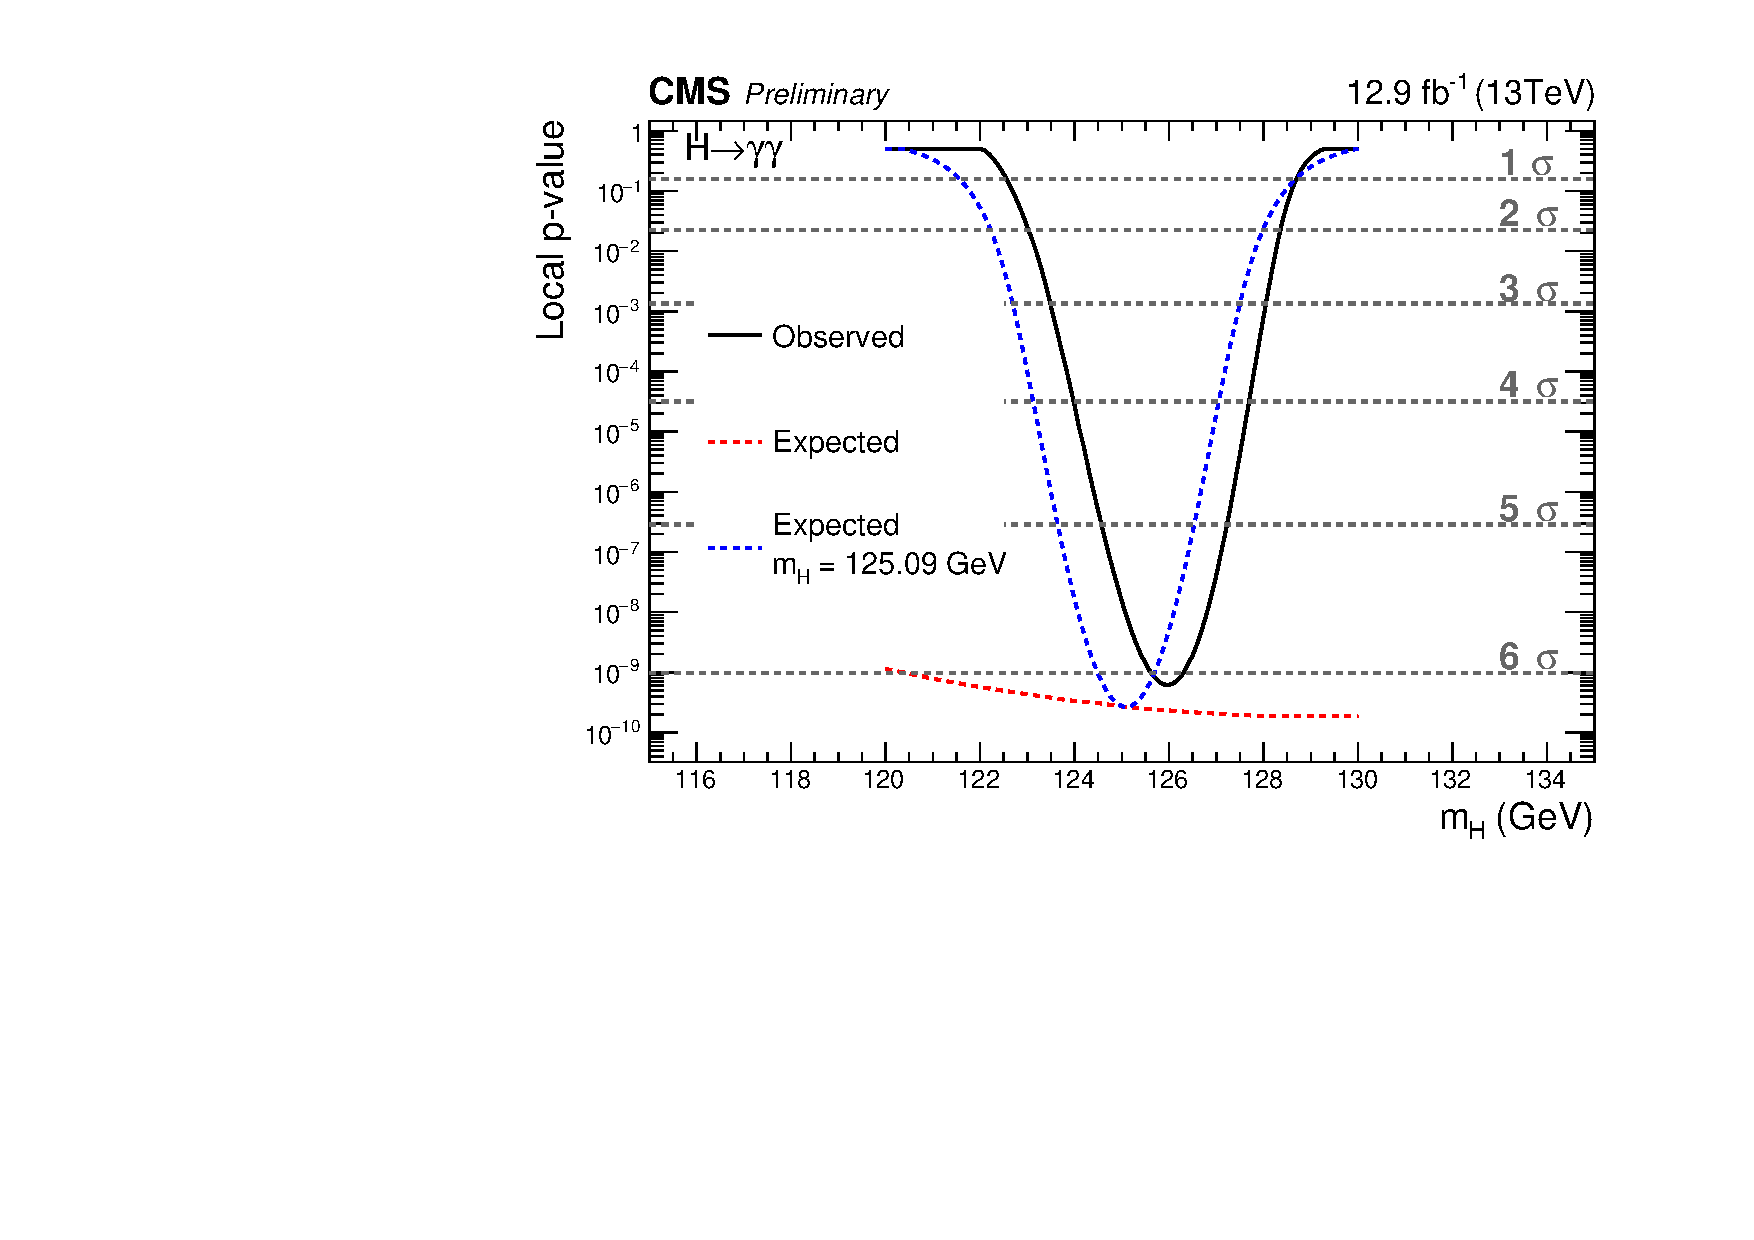
\includegraphics[width=0.9\textwidth]{statandresultsFigures/pval13TeV-observed.pdf} 
\caption{The \pvalue for the observation as a function of the Higgs boson mass (black), shown with the expected \pvalue\s for a \SM Higgs boson, across the range 120-130\GeV. The expected \pvalue\s are obtained using Asimov datasets~\cite{}. The blue line shows the expected \pvalue when the mass of the injected signal is $\mH=125.09\GeV$, while the red line shows the maximum significance for any injected signal in the range $120-1230\GeV$.}

\label{fig:statandresults:pval}
\end{figure}

\section{Measurements of the signal strength}
\subsection{Global signal strength}

One of the advantages of using \DNLL as a test statistic is that to a very good approximation, the $\pm 1 \sigma$ uncertainty on the measured value of the \POI, in this case $\mu$, can be obtained by finding the values of $\mu$ for which $q_{\mu}=q_{\hat{\mu}}+1$. ~\cite{}
This fact is used to produce a measurement of $\mu$. \Fig~\ref{fig:statandresults:global_mu} shows the value of the \DNLL is plotted as a function of fixed values of $\mu$. This is referred to as a likelihood scan. In this case, \mH is profiled as a nuisance parameter. By definition the best-fit point, $\hat{\mu}$ has a \DNLL value of $0$. This gives the central value for the measurement. The upper and lower uncertainties are obtained by graphically finding the intercepts of the curve with \DNLL$=1$. 
The contribution to the uncertainty on the signal strength from the statistical, theory systematic and experimental systematic components can be assessed by freezing the corresponding nuisance parameters. 
The measured value of the signal strength is $\hat{\mu}􏰋 = 0.95^{+0.21}_{-0.19} = 0.95 \pm 0.17 \text{ (stat.) } ^{0.09}_{-0.06} \text{ (theo. syst.) } ^{+0.10}_{-0.07} \text{ (exp. syst.) } $. This measurement indicates that the observed global signal strength is compatible with the \SM expectation within one standard deviation.

\begin{figure}[ht!]
\centering
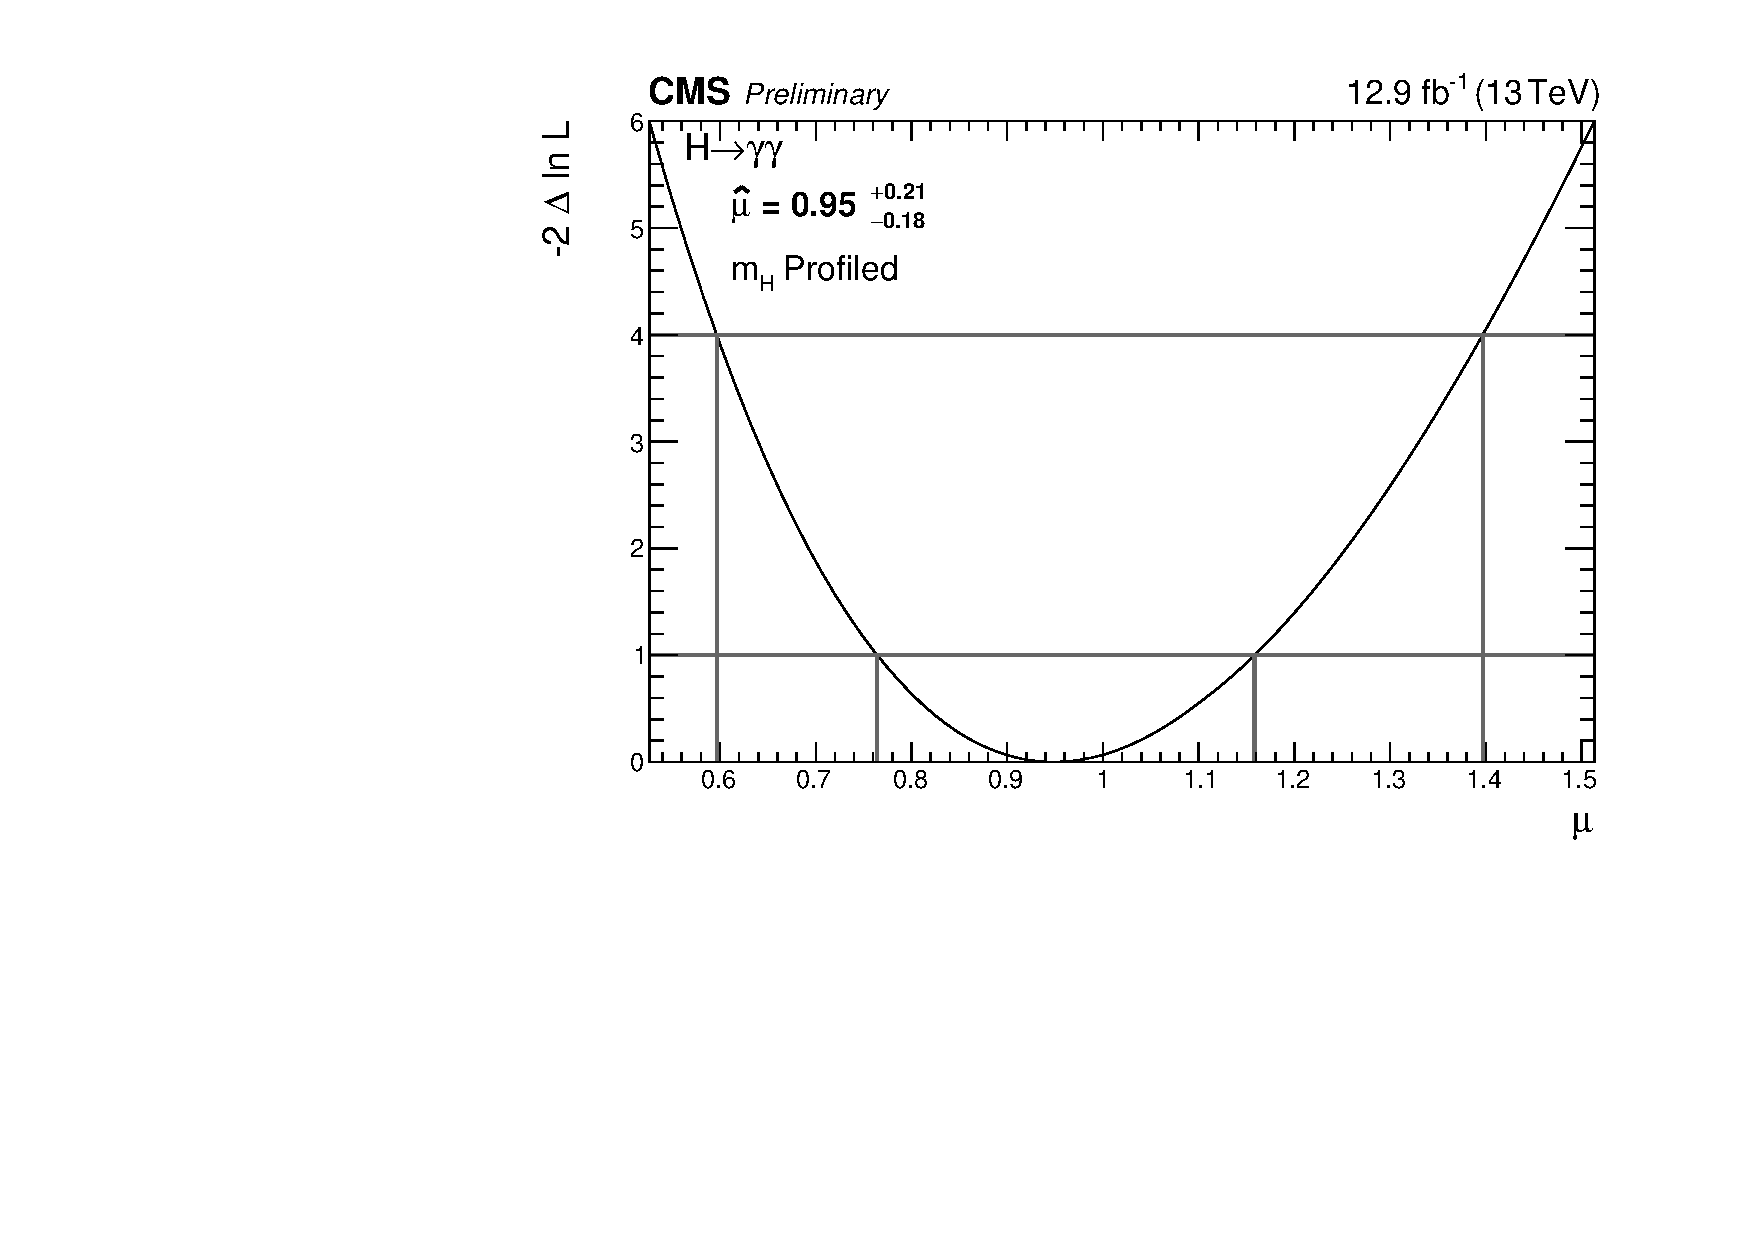
\includegraphics[width=0.9\textwidth]{statandresultsFigures/MuScanProfileMH.pdf} 
\caption{The likelihood scan of the overall signal strength for a Higgs boson decaying to two photons. The mass of the Higgs boson is treated as a nuisance parameter and profiled in the fit.}

\label{fig:statandresults:global_mu}
\end{figure}

Instead of profiling the \mH parameter, this can instead be fixed to particular values. A similar likelihood scan can be repeated for given values of \mH in the 120-1230\GeV range, in small steps. This is shown in \Fig~\ref{fig:statandresults:mu_vs_mh}, where the best fit signal strength is shown as function if the given \mH, where the green bands represent the $\pm 1 \sigma$ uncertainty obtained by finding the crossing with \DNLL$=1$.  

\begin{figure}[ht!]
\centering
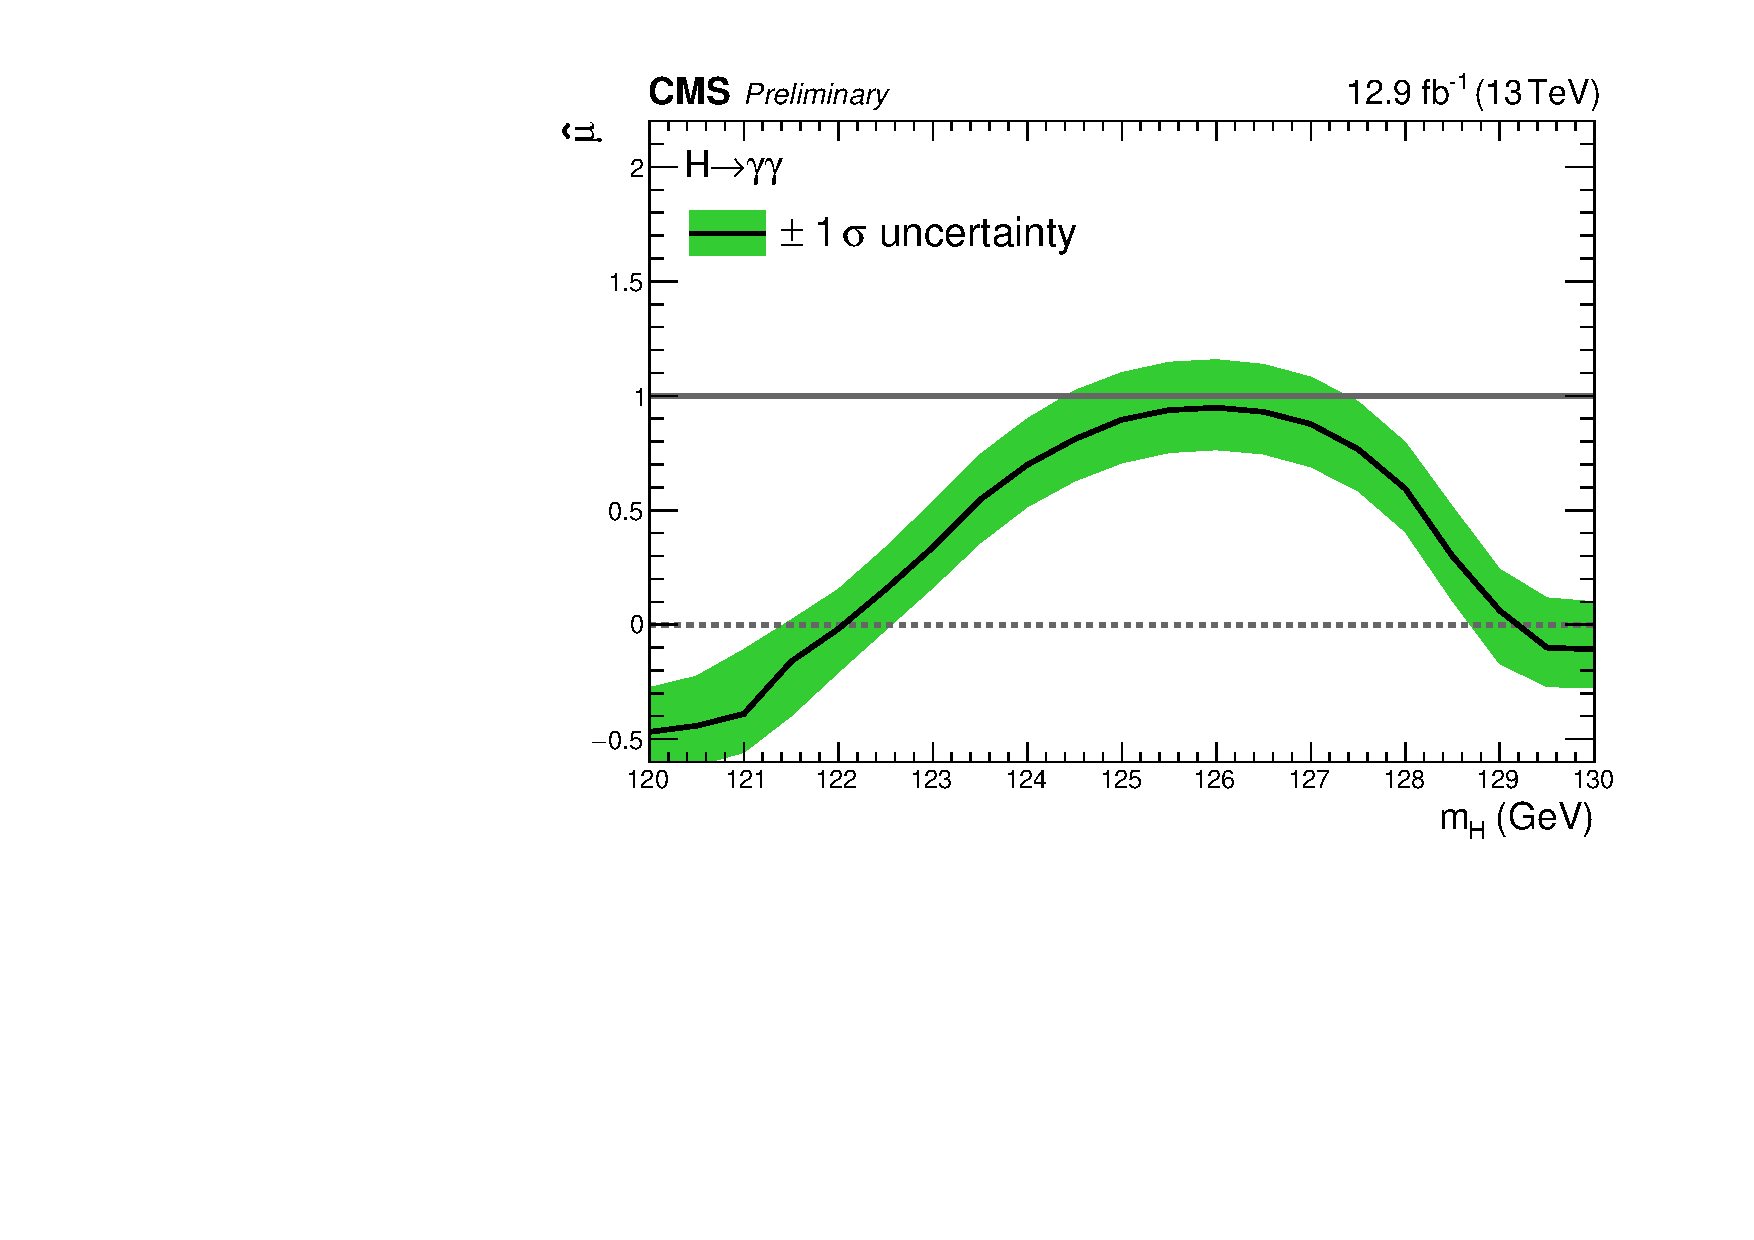
\includegraphics[width=0.9\textwidth]{statandresultsFigures/MuHat_vs_MH.pdf} 
\caption{The best-fit signal strength for fixed values of \mH in the 120-1230\GeV range, where the \mH parameter is fixed in the fitting procedure. The green bands show  the $\pm 1 \sigma$ uncertainty obtained by finding the crossing with \DNLL$=1$.  }

\label{fig:statandresults:mu_vs_mh}
\end{figure}

\subsection{Measurement of fermionic and bosonic components of the signal strength}
\label{sec:statandresults:rvrf}

When making the measurement of the signal strength in \Sec~\ref{Global signal strength}, a single \POI which uniformly scaled all production processes was assumed. However, the strategy makes the assumption that the relative contribution of each process to the total Higgs boson \crosssection is as predicted by the \SM. In order to test this assumption, the single \POI representing to global signal strength $\mu$ can be split up into its components. As a first stage, one can test whether the contributions from the production modes where the Higgs boson is produced from fermions (\ggH and \ttH) and bosons (\VBF and \VH) individually agree with the \SM expectation.

The measurement is made by producing a \DNLL scan with a slightly modified test statistics, where we now consider two \POI\s, \muF and \muV. The \muF parameter scales the yield of the signal models for the \ggH and \ttH processes in all categories uniformly, but does not affect the yields of the models for the \VBF or \VH processes, and vie-versa for the \muV parameter. The \mH parameter is profiled in the two-dimensional \DNLL scan.

The results of the scan can be seen in \Fig~\ref{}. The $z$-axis, representing the value of \DNLL, has been omitted for clarity.  The black cross shows the location of the best-fit point, with the red diamond indicating the \SM expectation. The $1\sigma$ and $2\sigma$ contours, which represent the intercepts of the two-dimensional \DNLL curve with $\DNLL=2.30$ and $\DNLL=6.18$ respectively, are shown in dashed lines. The plot shows that the observation is consistent with the \SM hypothesis within $1\sigma$.
\begin{figure}[ht!]
\centering
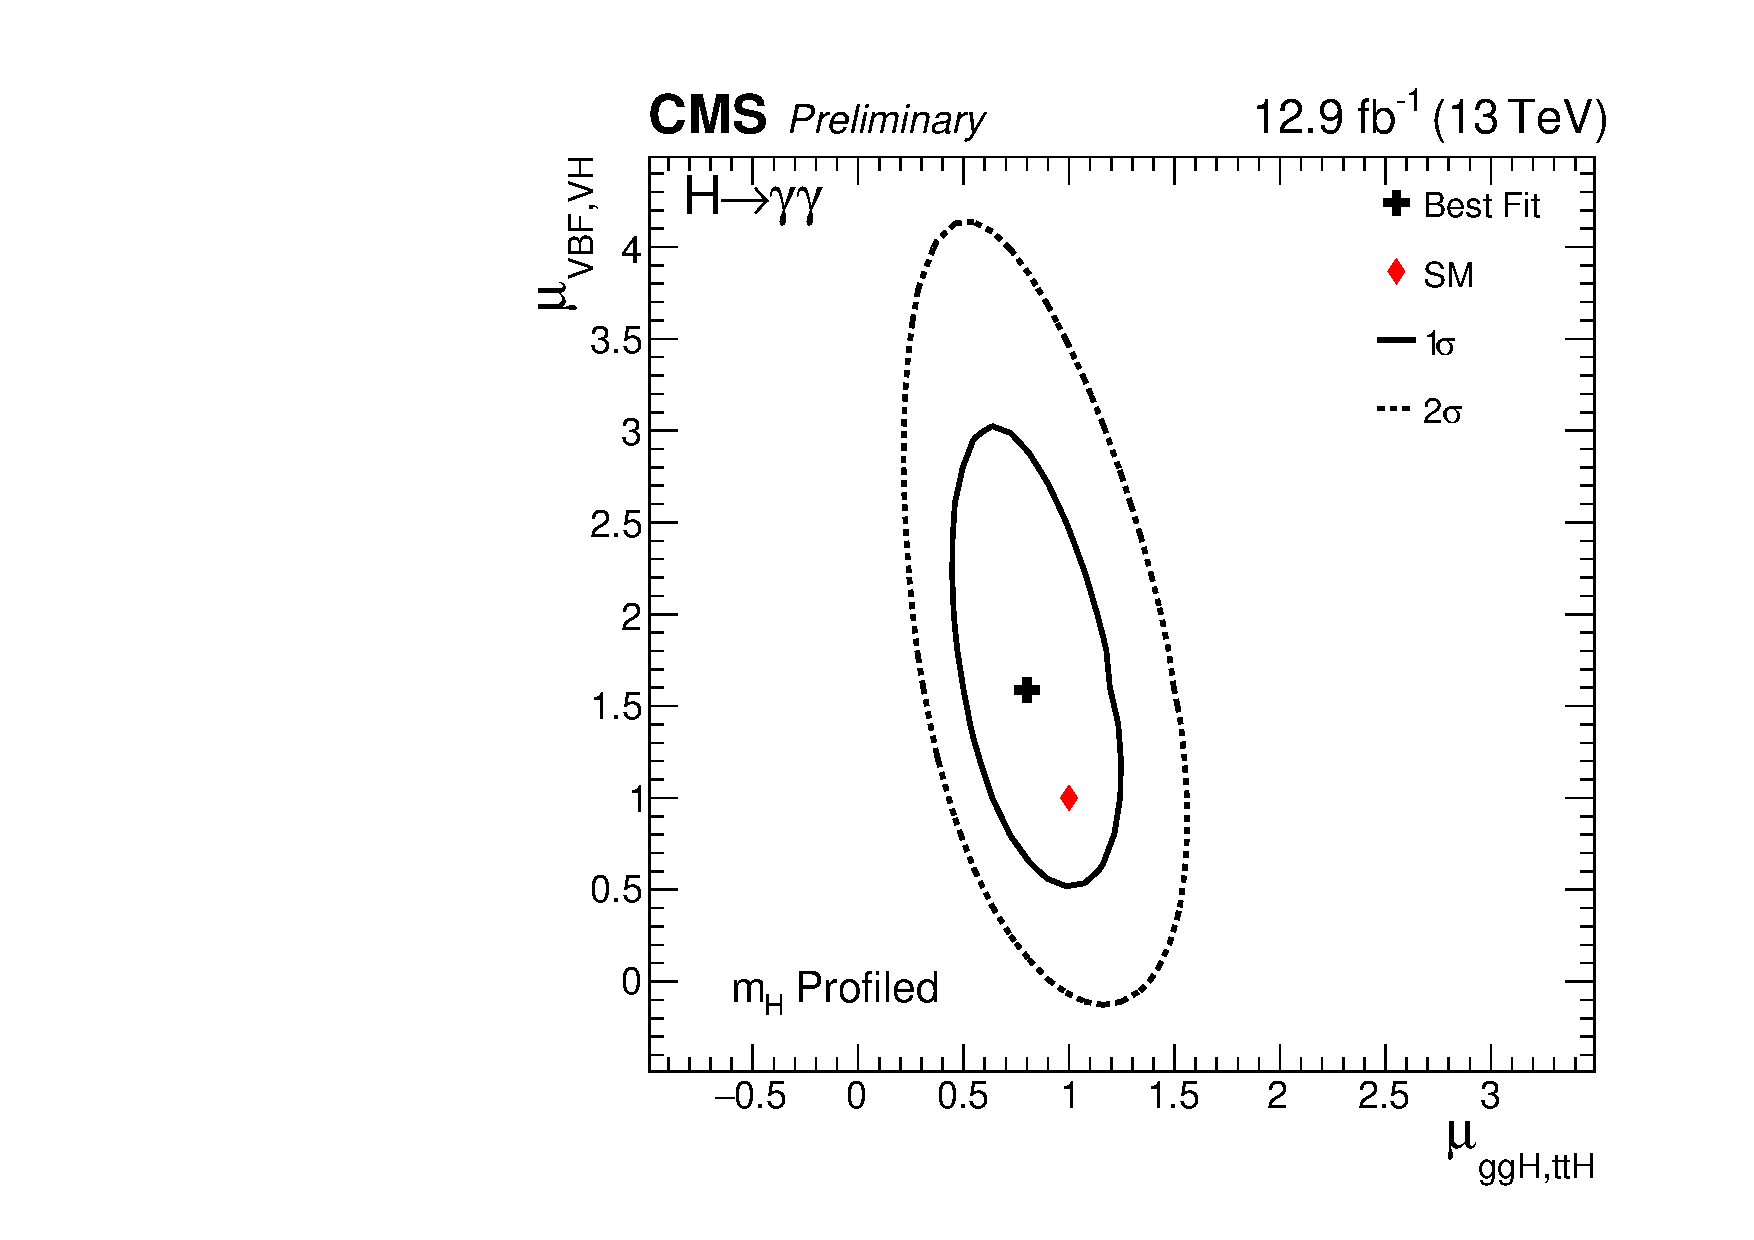
\includegraphics[width=0.9\textwidth]{statandresultsFigures/RVRFScanProfileMH.pdf} 
\caption{The result of a two-dimensional -2$\Delta$NLL scan of the \muF and \muV components of the signal strength. The red star indicates the \SM expectation, while the black cross shows the location of the best fit point. The measurement is consistent with the \SM within the uncertainty contours, which are shown in dashed lines. The value of \mH was profiled in these scans.}

\label{fig:statandresults:mu_per_rvrf}
\end{figure}

To make measurements of \muF and \muV individually, a log-likelihood scan of each is performed while profiling the other. The resulting scans can be seen in \Fig\s~\ref{} and ~\ref{}. The result of the measurement is found to be $\hat{\muF}=0.75{+0.31}_{-0.12}$ and $\hat{\muV}=1.49{+0.90}_{-0.0.73}$. The fermionic and bosonic components of the Signal strength are therefore found to be compatible with the \SM expectations. 

\begin{figure}[ht!]
\centering
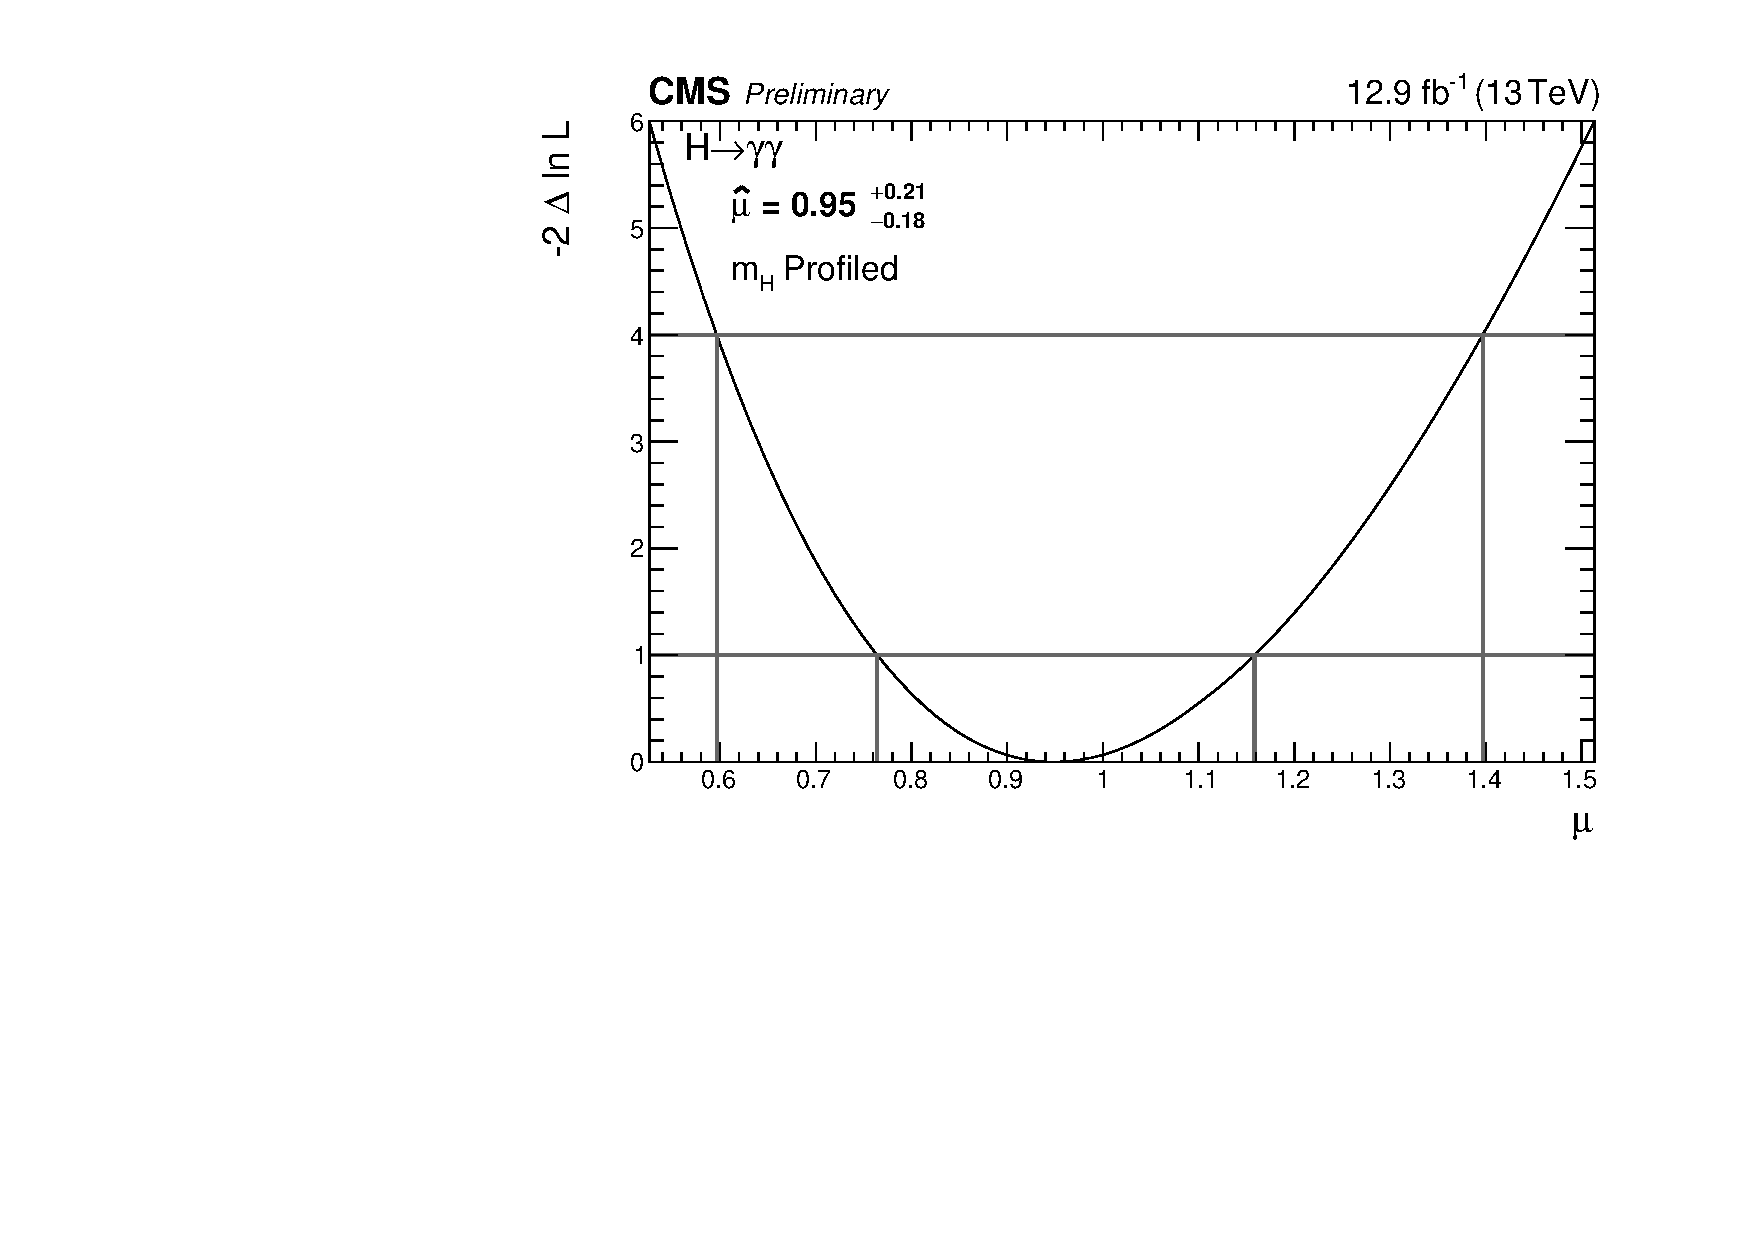
\includegraphics[width=0.7\textwidth]{statandresultsFigures/MuScanProfileMH.pdf} \\
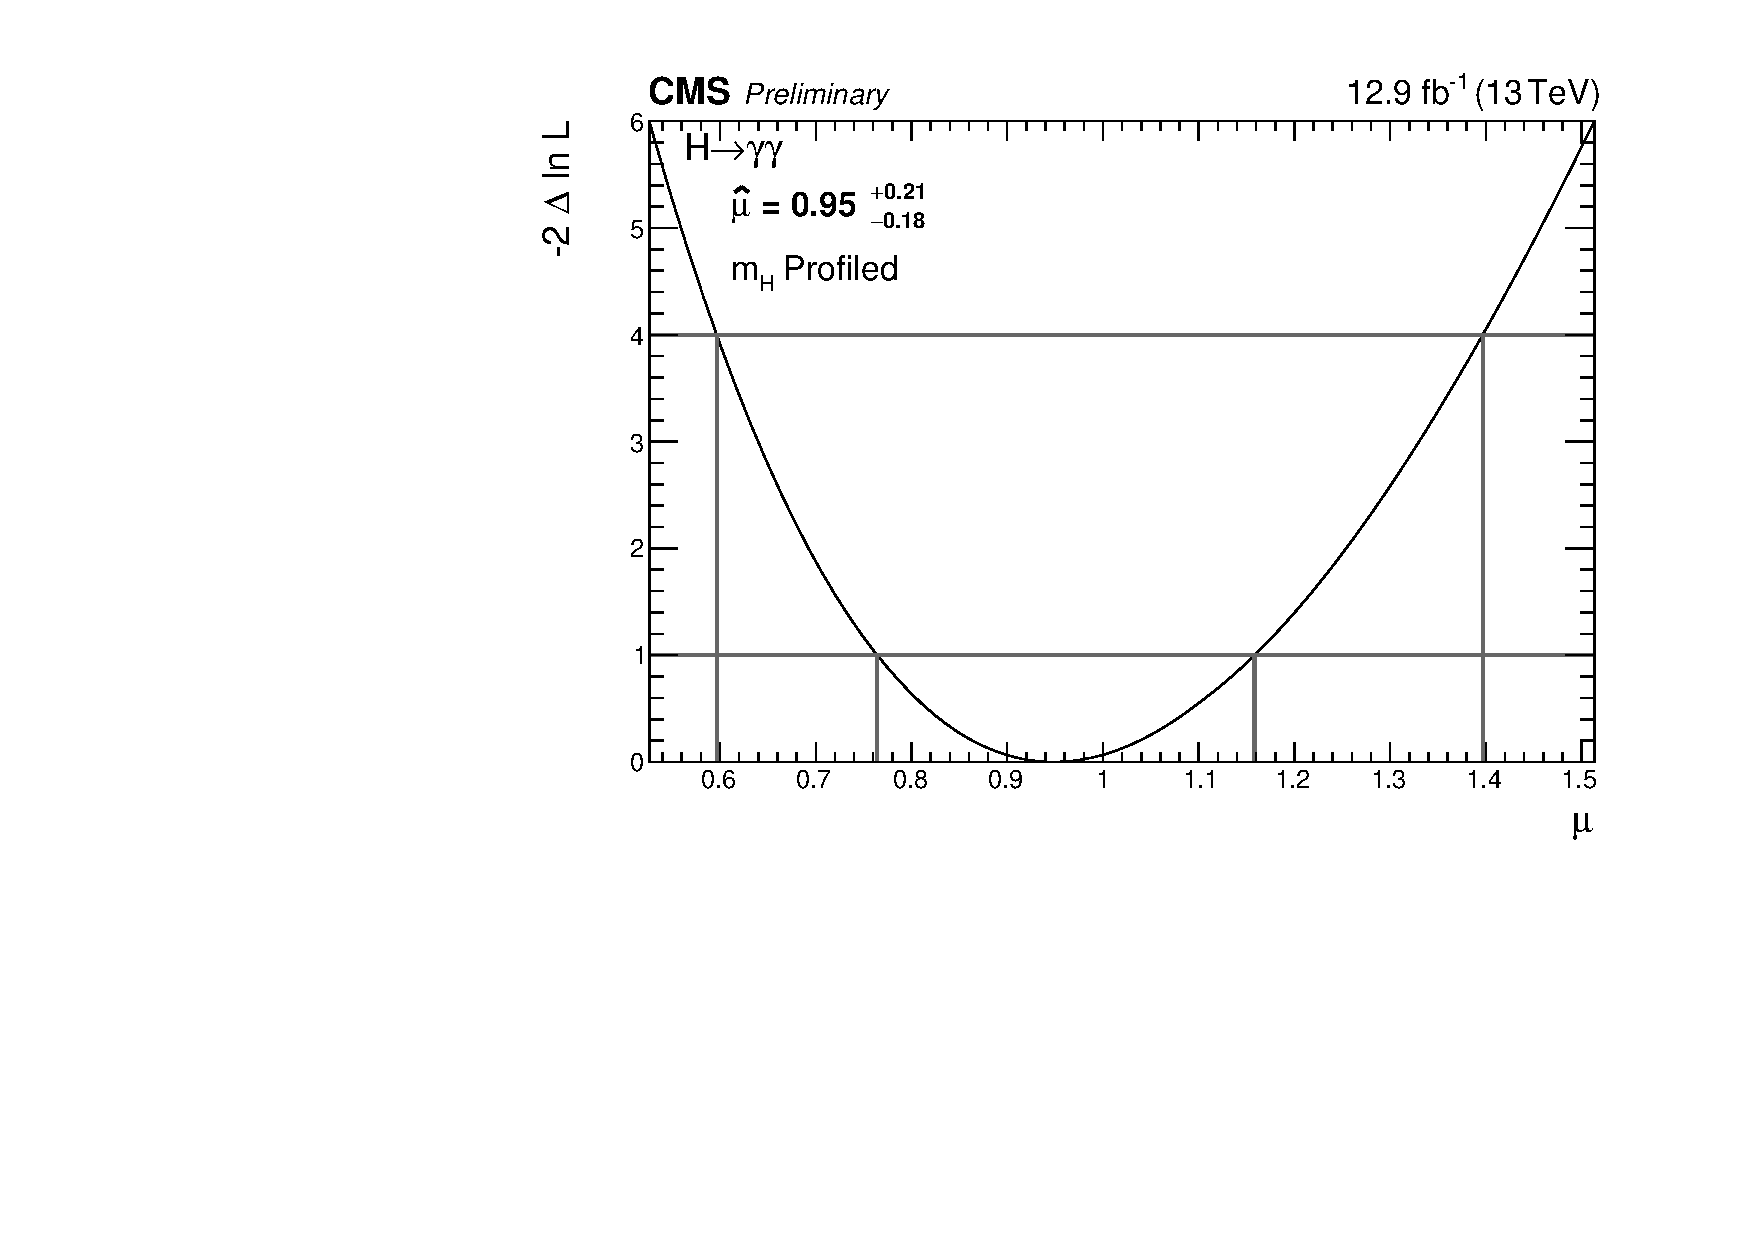
\includegraphics[width=0.7\textwidth]{statandresultsFigures/MuScanProfileMH.pdf} 
\caption{The result of performing a -2$\Delta$NLL scans of \muF while profiling \muV (a) and vice-versa (b). In both cases the mass of the Higgs boson is profiled in the fit. }

\label{fig:statandresults:mu_per_rv_and_rf}

\end{figure}

\subsection{Individual signal strengths of each process}

Using a similar procedure to what was described in \Sec~\ref{sec:statandresults:rvrf}, measurements of the signal strengths of the individual Higgs boson production modes (\muggH, \muVBF, \muVH, and \muttH) can be made. In this case, the test statistic is modified to contain one \POI for each production mode. The individual per-process signal strengths independently scale the signal yield of each process in all categories at once. This measurement is possible because it exploits categorisation scheme described in \Sec~\ref{}: the fact that the categories have a different composition in terms of contribution from different processes, allows the strength of the signal for each process to be differentiated. However, by the same logic, since no \VHTag categories are included in this analysis, it is not possible to resolve the \VH process from other processes, in particular \ggH since most \VH events are included in the \Untagged categories along with \ggH. Therefore, when making the measurements of the other \POI\s, the parameter \muVH is fixed to a value of 1. The measurements of the \muggH, \muVH, and \muttH are performed by producing a \DNLL scan of each one, while profiling the others. The \mH parameter is also profiled. The best-fit values and their uncertainties are shown on \Fig~\ref{}. The overall result obtained as described in \Sec~\ref{} is shown as the vertical line with green bands for the uncertainties. The \SM expectation is shown as the dashed red line. The per-process signal strength measurements are all compatible with the \SM expectation.

\begin{figure}[ht!]
\centering
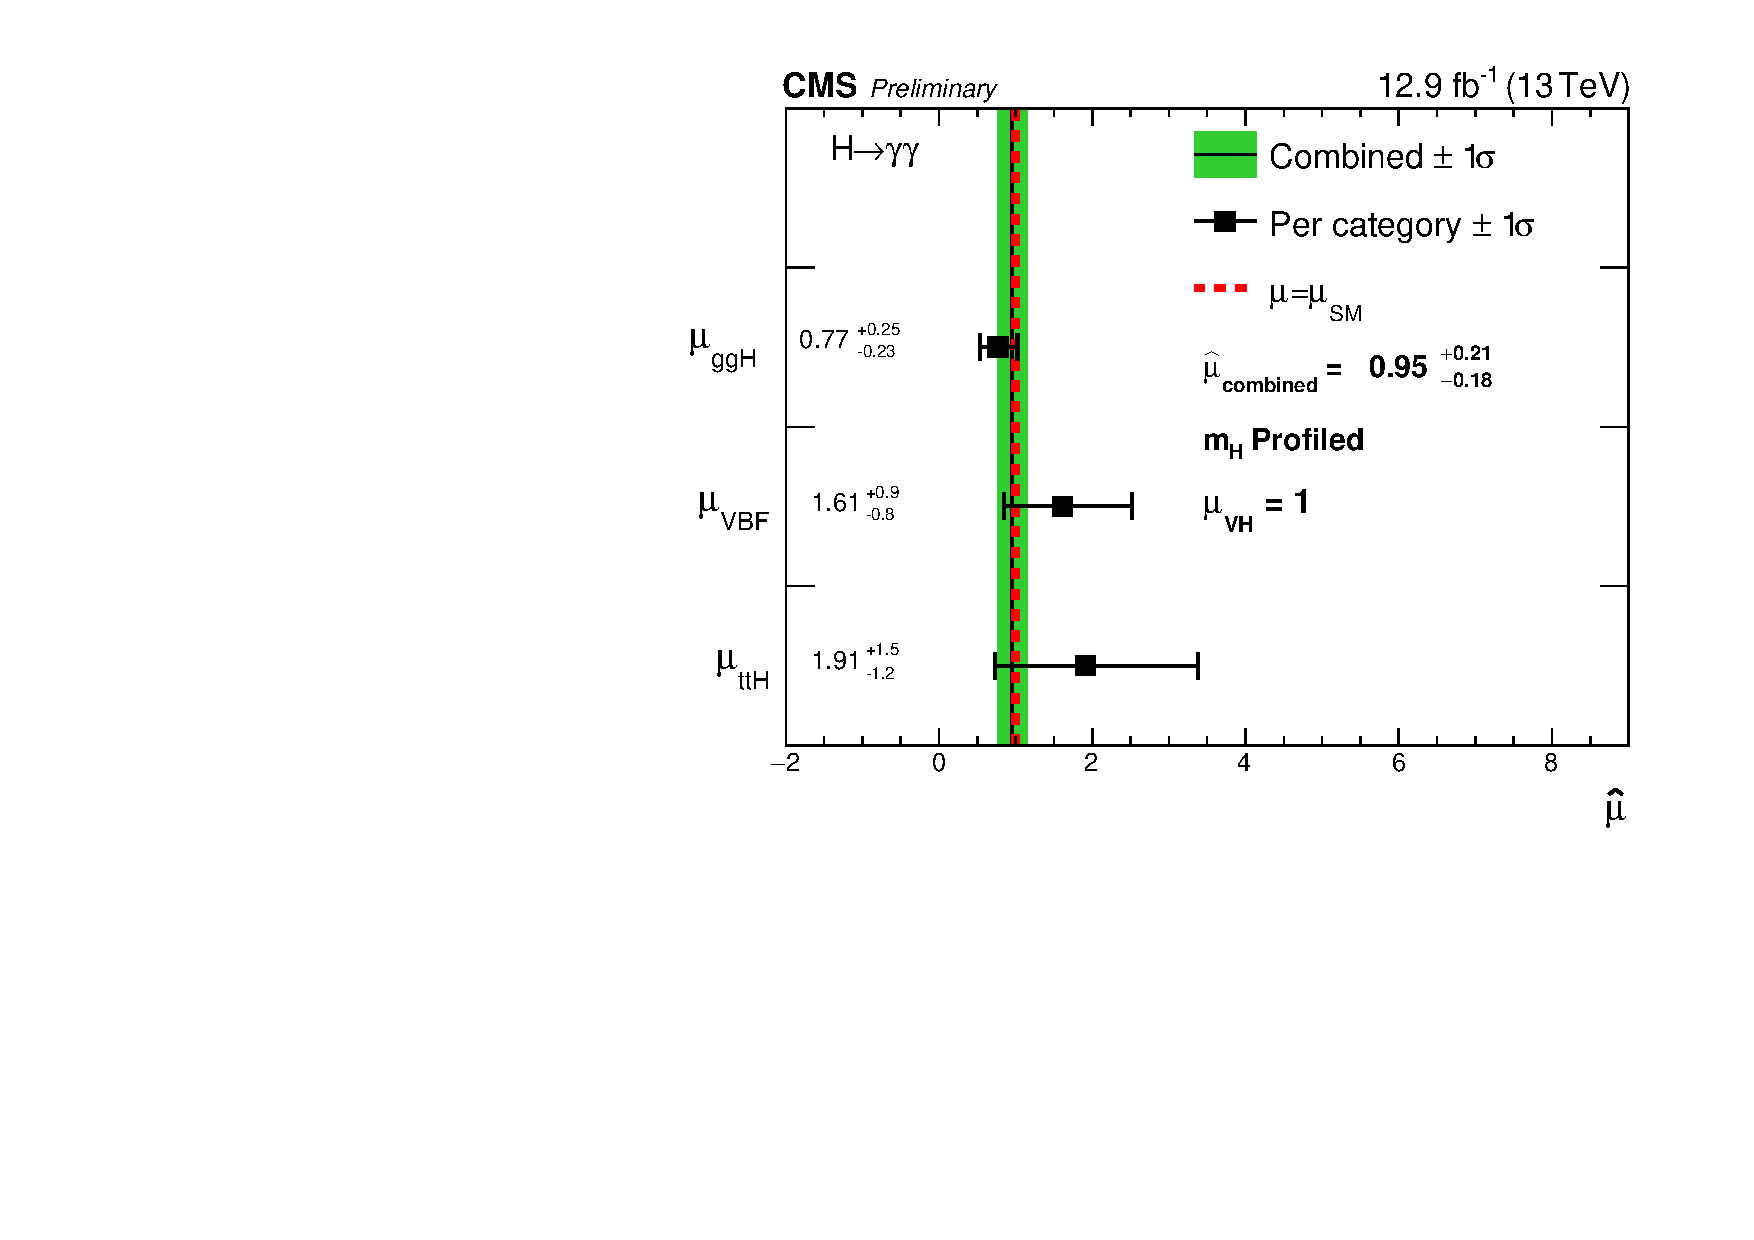
\includegraphics[width=0.9\textwidth]{statandresultsFigures/PerProcChannelCompatibilityProfileMH.pdf} 
\caption{The measurements of the per-process signal strengths \muggH, \muVBF, \muttH, obtained by performing \DNLL scans of each one while profiling the others. In each case \mH is also profiled in the fit, and $\muVH=1$ is imposed since this analysis foes not include any categories specifically targeting the \VH process. The vertical black line and green bands represent the measurement of the overall signal strength $\mu$, and the \SM expectation is shown in the vertical red dashed line.}

\label{fig:statandresults:mu_per_proc}

\end{figure}

\subsection{Compatibility of result with SM in each category}

Using a method very similar to the that described in \Sec~\ref{}, it is possible to make a measurement of the signal strength in each category separately. In this case, one signal strength per analysis category is defined, which scales the yield of the signal models of all processes uniformly, but independently within each category. Although the per-category signal strengths do not have any physical meaning, they are important checks that each category gives a result consistent with the overall measurement, and that no bias is introduced by any particular category. The result of the check is shown in \Fig~\ref{}, which determines that all the per-category signal strengths are compatible with the \SM expectation and the overall result.

\begin{figure}[ht!]
\centering
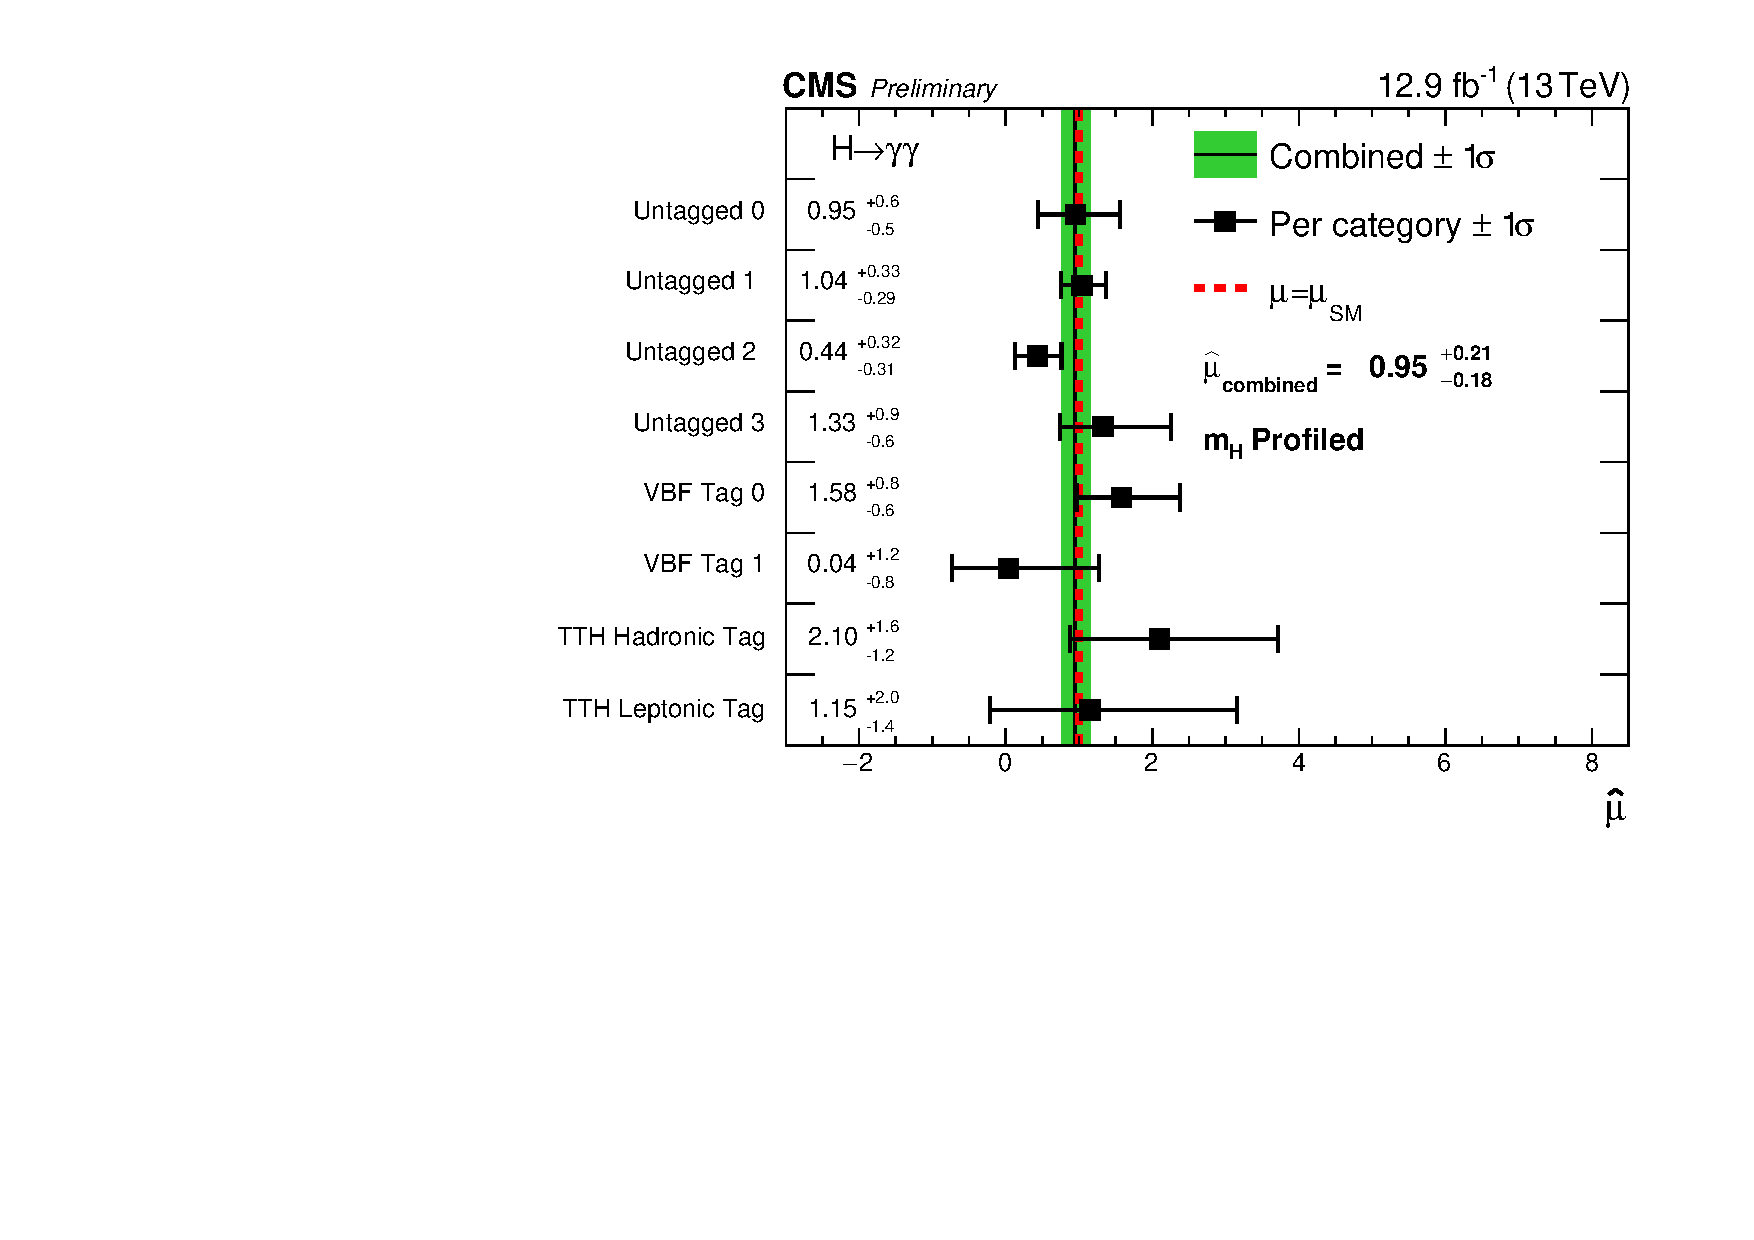
\includegraphics[width=0.9\textwidth]{statandresultsFigures/PerTagChannelCompatibilityProfileMH.pdf} 
\caption{The measurements of the per-category signal strengths, obtained by performing \DNLL scans of each one while profiling the others. In each case \mH is also profiled in the fit, The vertical black line and green bands represent the measurement of the overall signal strength $\mu$, and the \SM expectation is shown in the vertical red dashed line. The per-category signal strengths are not meaningful physical observables, and this result is a check that no particular category is introducing a large bias into the overall measurement.}

\label{fig:statandresults:mu_per_tag}

\end{figure}

\section{Measurements of Higgs boson coupling modifiers ($\kappa$)}

The measurements presented so far have all been variations of the Higgs boson signal strength. Such observables are sensitive the variations in the rate at which the Higgs boson is produced, before decaying (in this case into a pair of photons). An alternative set of measurements can be made, which are instead sensitive to variations in the coupling strength  of the Higgs boson with individual particles, relative to the \SM expectation.The so-called \emph{kappa} framework assigns a modifier to the coupling strength of the Higgs boson to a particle or group of particles $X$ and is labelled as $\kappa_{X}$~\cite{}. The coupling of the Higgs boson to massless particles can only occur indirectly, so these are probed in terms of modifiers to the effective coupling. 
The assumptions which underly this framework are as follows: 
\begin{itemize}
\item any calculated deviations from the \SM are due to only one Higgs-boson-like state with mass around 125\GeV;
\item the natural width of this state is sufficiently small that it can be neglected, allowing the \crosssection and branching fraction for a process $ii\rightarrow H \rightarrow ff$ to be decomposed as $(\sigma_{ii}^{H} \cdot \Gamma_{ff}^{H}) / (\Gamma_H)$, where is $\sigma_{ii}^{H}$ the \crosssection for a Higgs boson to be produced from the initial state $ii$,  $\Gamma^{H}_{ff}$ is the partial decay width of the Higgs boson into the state $ff$ and $\Gamma_{H}$ is the total width of the Higgs boson.
\end{itemize}

The coupling modifier  $\kappa_{X}$ for a particle $X$ interacting with the Higgs boson is applied directly as a modified to the corresponding $\sigma_{XX}^{H}$ if the interaction produces a Higgs boson or $\Gamma^{H}_{XX}$ if the interaction involves the decay of  a Higgs boson. For processes which only occur via loops of particles, i.e. \Hgg, the effective coupling is defined as a function of the particles in which play a large role, i.e. $\kappa_{\gamma} = \kappa_{\gamma}(\kappa_b, \kappa_t,\kappa_\tau,\kappa_W) $ and $\kappa_{g} = \kappa_{\gamma}(\kappa_b, \kappa_t) $. In this case, we consider a  coupling modifier $\kf$ ($\kV$)which uniformly scales the coupling strength modifier for all fermions (fermions). The results of a two-dimensional \DNLL scan of \kf and \kV is shown in \Fig~\ref{fig:statandresults:kappa_plots_kvkf}, where the \mH parameter was profiled in the fit. The black cross indicates the best-fit while the red star indicates the \SM expectation. The $1\sigma$ and $2\sigma$ contours are indicated by dashed lines. The best-fit indicates compatibility with the \SM. An interesting feature of this plot is that a second local minimum exists where \kf takes negative values. In general, the coupling strength modifiers always occur squared in the amplitude, but interference effects can give a small sensitivity to the sign of some coupling strength modifiers. The best-fit point agrees with the \SM within the uncertainties.

\begin{figure}[ht!]
\centering
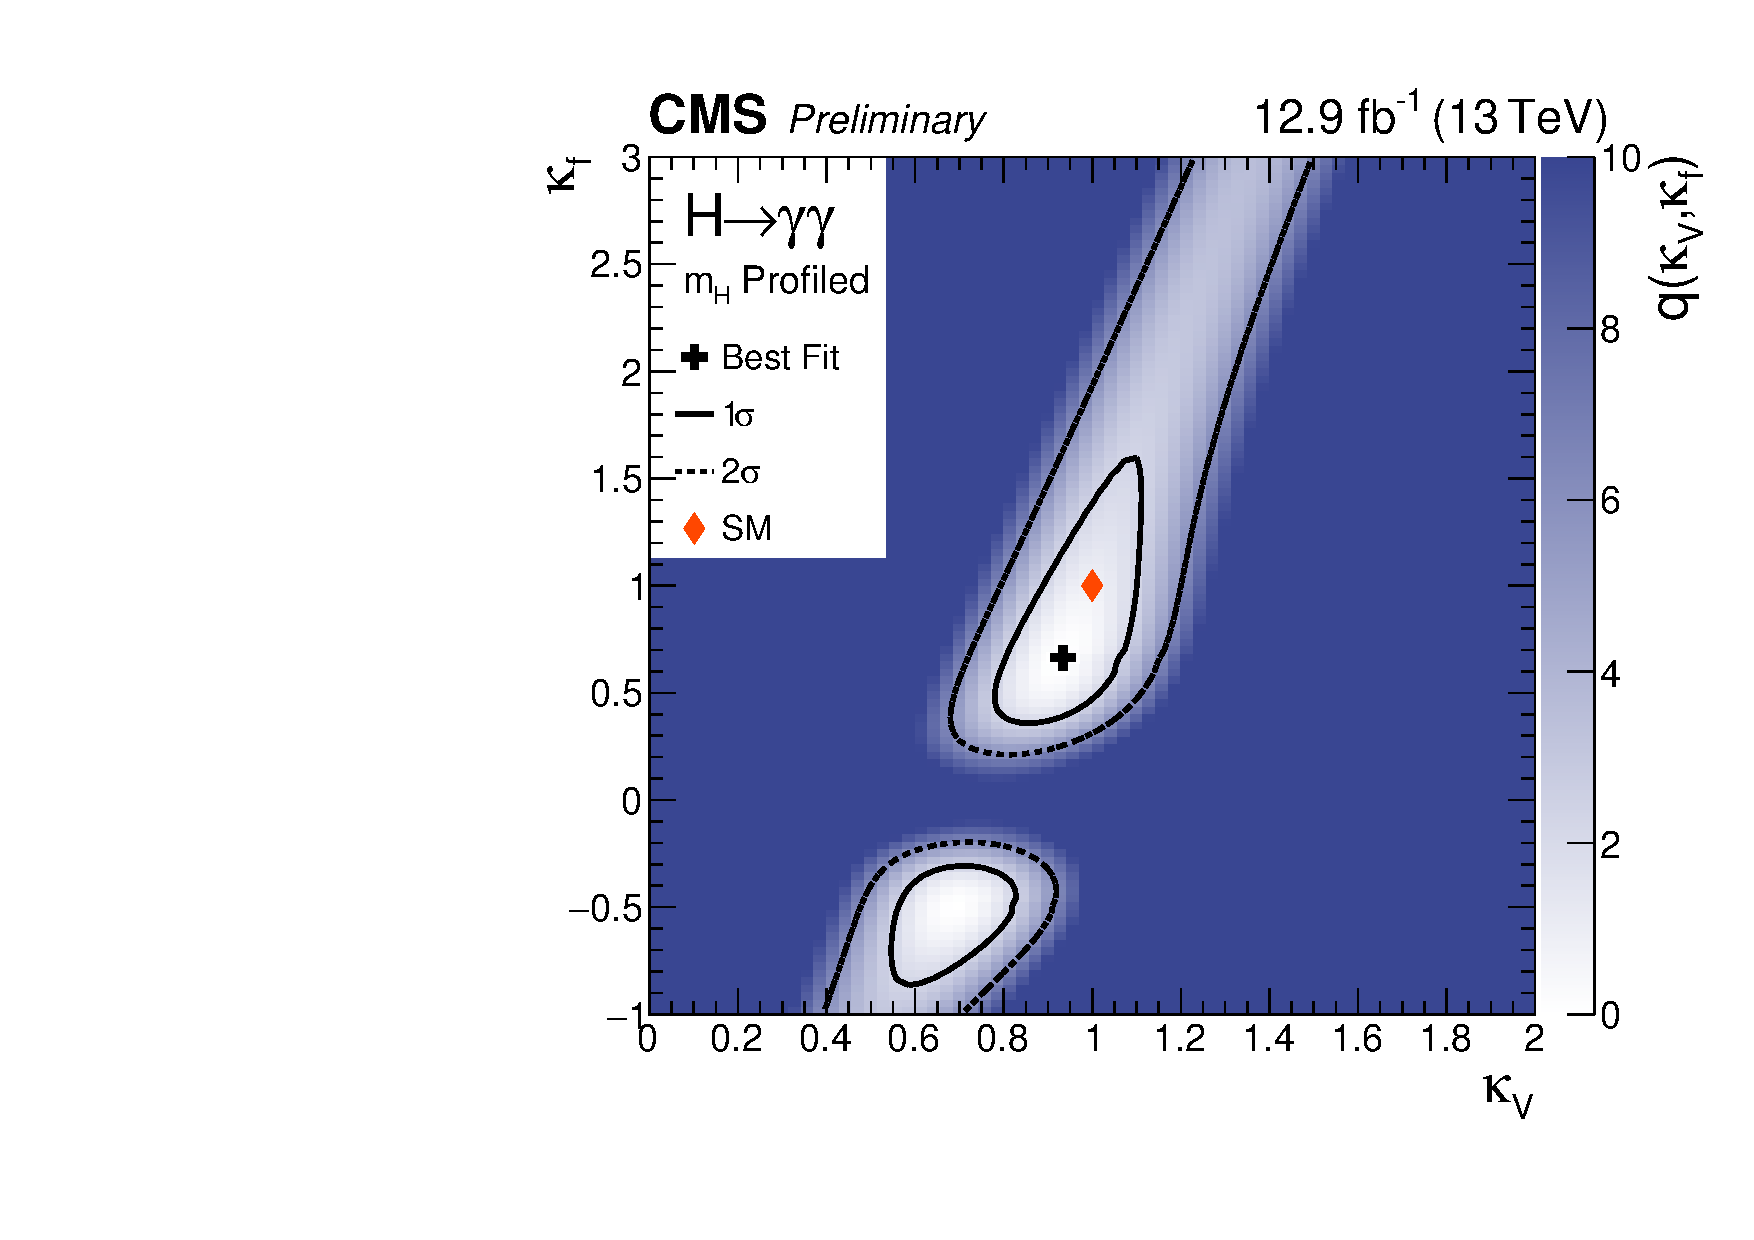
\includegraphics[width=0.7\textwidth]{statandresultsFigures/CVCFScanProfileMH_granular_col.pdf} 
\caption{The result of a two-dimensional -2$\Delta$NLL scan of the coupling strength modified for fermions (\kf) and vector bosons (\kV). The best fit value is denoted with a black cross and the \SM expected value with a red diamond. The best-fit agrees with the \SM within the uncertainty contours denoted by dashed lines. }

\label{fig:statandresults:kappa_plots_kvkf}
\end{figure}

Alternatively, measurements can be made of the Higgs boson's effective coupling to gluons (\kGlu) and photons (\kPho) using a \DNLL scan where the \mH parameter was profiled. The results are presented in \Fig~\ref{fig:statandresults:kappa_plots_kgkg}. The best-fit point agrees with the \SM within the uncertainties.


\begin{figure}[ht!]
\centering
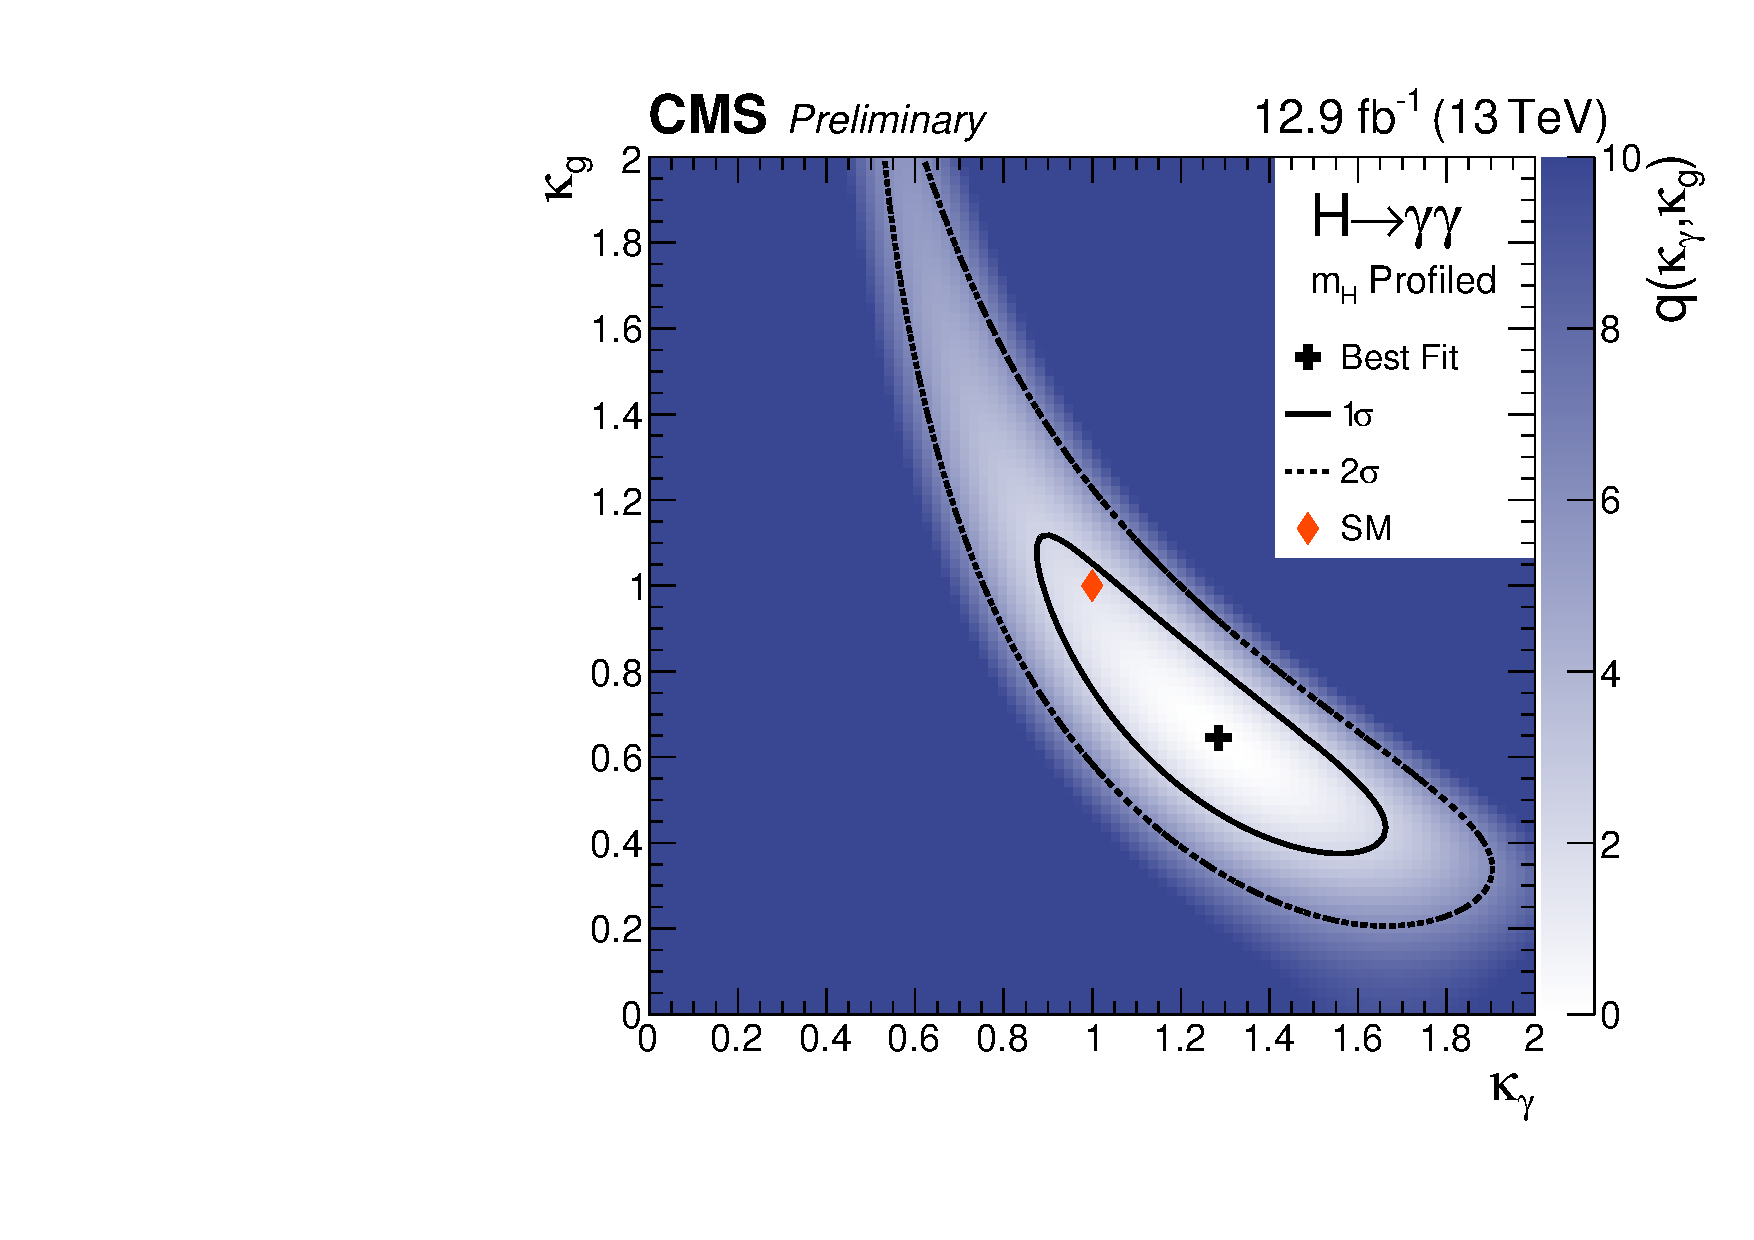
\includegraphics[width=0.7\textwidth]{statandresultsFigures/KGluKGamScanProfileMH_granular_col.pdf} 
\caption{The result of a two-dimensional -2$\Delta$NLL scan of the effective coupling strength modified for gluons (\kGlu) and photons (\kPho). The best fit value is denoted with a black cross and the \SM expected value with a red diamond. The best-fit agrees with the \SM within the uncertainty contours denoted by dashed lines. }

\label{fig:statandresults:kappa_plots_kgkp}

\end{figure}
